% ptop: how the program works. Page 1 is the overview, the other pages show one or two functions each.
% Build:            pdflatex ptop-flow.tex
% PNGs for README:  pdftoppm -png -r 150 ptop-flow.pdf ptop-flow   (one file per page)
%
% Skip epstopdf: a minimal TinyTeX lacks grfext, and these diagrams have no EPS images
\def\DoNotLoadEpstopdf{}
\documentclass[tikz,border=12pt]{standalone}
\usepackage[T1]{fontenc}
\usepackage{lmodern}
\usepackage{amsmath}
\usetikzlibrary{positioning,fit,arrows.meta,backgrounds,calc,shapes.geometric}

\definecolor{readc}{HTML}{2F6FB0}
\definecolor{compc}{HTML}{2E8B57}
\definecolor{printc}{HTML}{C0602A}
\definecolor{ttyc}{HTML}{7B4FA0}
\definecolor{basec}{HTML}{4A4A4A}

% Function name in monospace, underscores allowed (no % # or backslash-letter inside)
\newcommand{\fn}[1]{\texttt{\detokenize{#1}}}
% Escape sequence written as in the C source
\newcommand{\esc}[1]{\texttt{\textbackslash x1b#1}}
% Short note under a step
\newcommand{\nt}[1]{{\scriptsize\itshape\color{black!62}#1}}
% Circled number: the order to revise in
\newcommand{\st}[1]{\tikz[baseline=(c.base)]\node[circle,draw=black!55,fill=white,
    inner sep=0.5pt,minimum size=3.6mm,font=\scriptsize\bfseries](c){#1};}
% One function in a stage box on page 1: number, name, a few words
\newcommand{\entry}[3]{\st{#1}\;\textbf{\fn{#2}}\\[-1pt]{\footnotesize\color{black!72}#3}\\[4pt]}

\tikzset{
  >={Stealth[length=2.3mm,width=1.7mm]},
  every node/.style={font=\small},
  % page 1
  stage/.style={draw=#1, fill=#1!6, rounded corners=4pt, line width=0.9pt,
                align=left, text width=5.5cm, inner sep=7pt, inner ysep=9pt, anchor=north},
  tab/.style={fill=#1, text=white, font=\bfseries\small, rounded corners=3pt,
              inner xsep=6pt, inner ysep=3pt, anchor=west},
  pill/.style={draw=#1, fill=#1!16, rounded corners=7pt, line width=0.9pt,
               font=\small\bfseries, minimum height=6.5mm, minimum width=20mm, align=center},
  step/.style={draw=#1, fill=white, rounded corners=3pt, line width=0.8pt,
               align=left, inner sep=4pt},
  frame/.style={draw=#1, rounded corners=6pt, dashed, line width=0.8pt},
  flow/.style={->, line width=0.8pt, draw=black!65, rounded corners=3pt},
  lbl/.style={font=\scriptsize, text=black!75, fill=white, inner sep=1.5pt},
  % function pages
  pagehead/.style={font=\Large\bfseries, anchor=west, text=black!85},
  ftitle/.style={fill=#1, text=white, rounded corners=4pt, font=\bfseries\small,
                 inner xsep=8pt, inner ysep=5pt, align=center},
  act/.style={draw=black!55, fill=white, line width=0.7pt, rounded corners=1.5pt,
              align=center, text width=5cm, inner sep=4pt, font=\footnotesize},
  call/.style={act, draw=#1, fill=#1!10, line width=0.8pt},
  ask/.style={diamond, aspect=2.6, draw=black!55, fill=yellow!14, line width=0.7pt,
              align=center, inner sep=0.5pt, font=\footnotesize},
  good/.style={draw=green!45!black, fill=green!10, rounded corners=7pt, line width=0.8pt,
               align=center, inner sep=4pt, font=\footnotesize},
  bad/.style={draw=red!60!black, fill=red!8, rounded corners=7pt, line width=0.8pt,
              align=center, inner sep=4pt, font=\footnotesize},
  side/.style={draw=black!25, fill=black!3, rounded corners=3pt, align=left,
               text width=#1, inner sep=6pt, font=\footnotesize},
  side/.default=5cm,
  ex/.style={font=\ttfamily\small, inner xsep=1.6pt, inner ysep=2pt},
  exl/.style={font=\scriptsize, text=black!75, align=center, anchor=north},
  cell/.style={draw=black!50, minimum width=6mm, minimum height=6mm, line width=0.6pt},
}

\begin{document}
\hyphenpenalty=10000 \exhyphenpenalty=10000

%% ====================================================================
%% Page 1: overview
%% ====================================================================
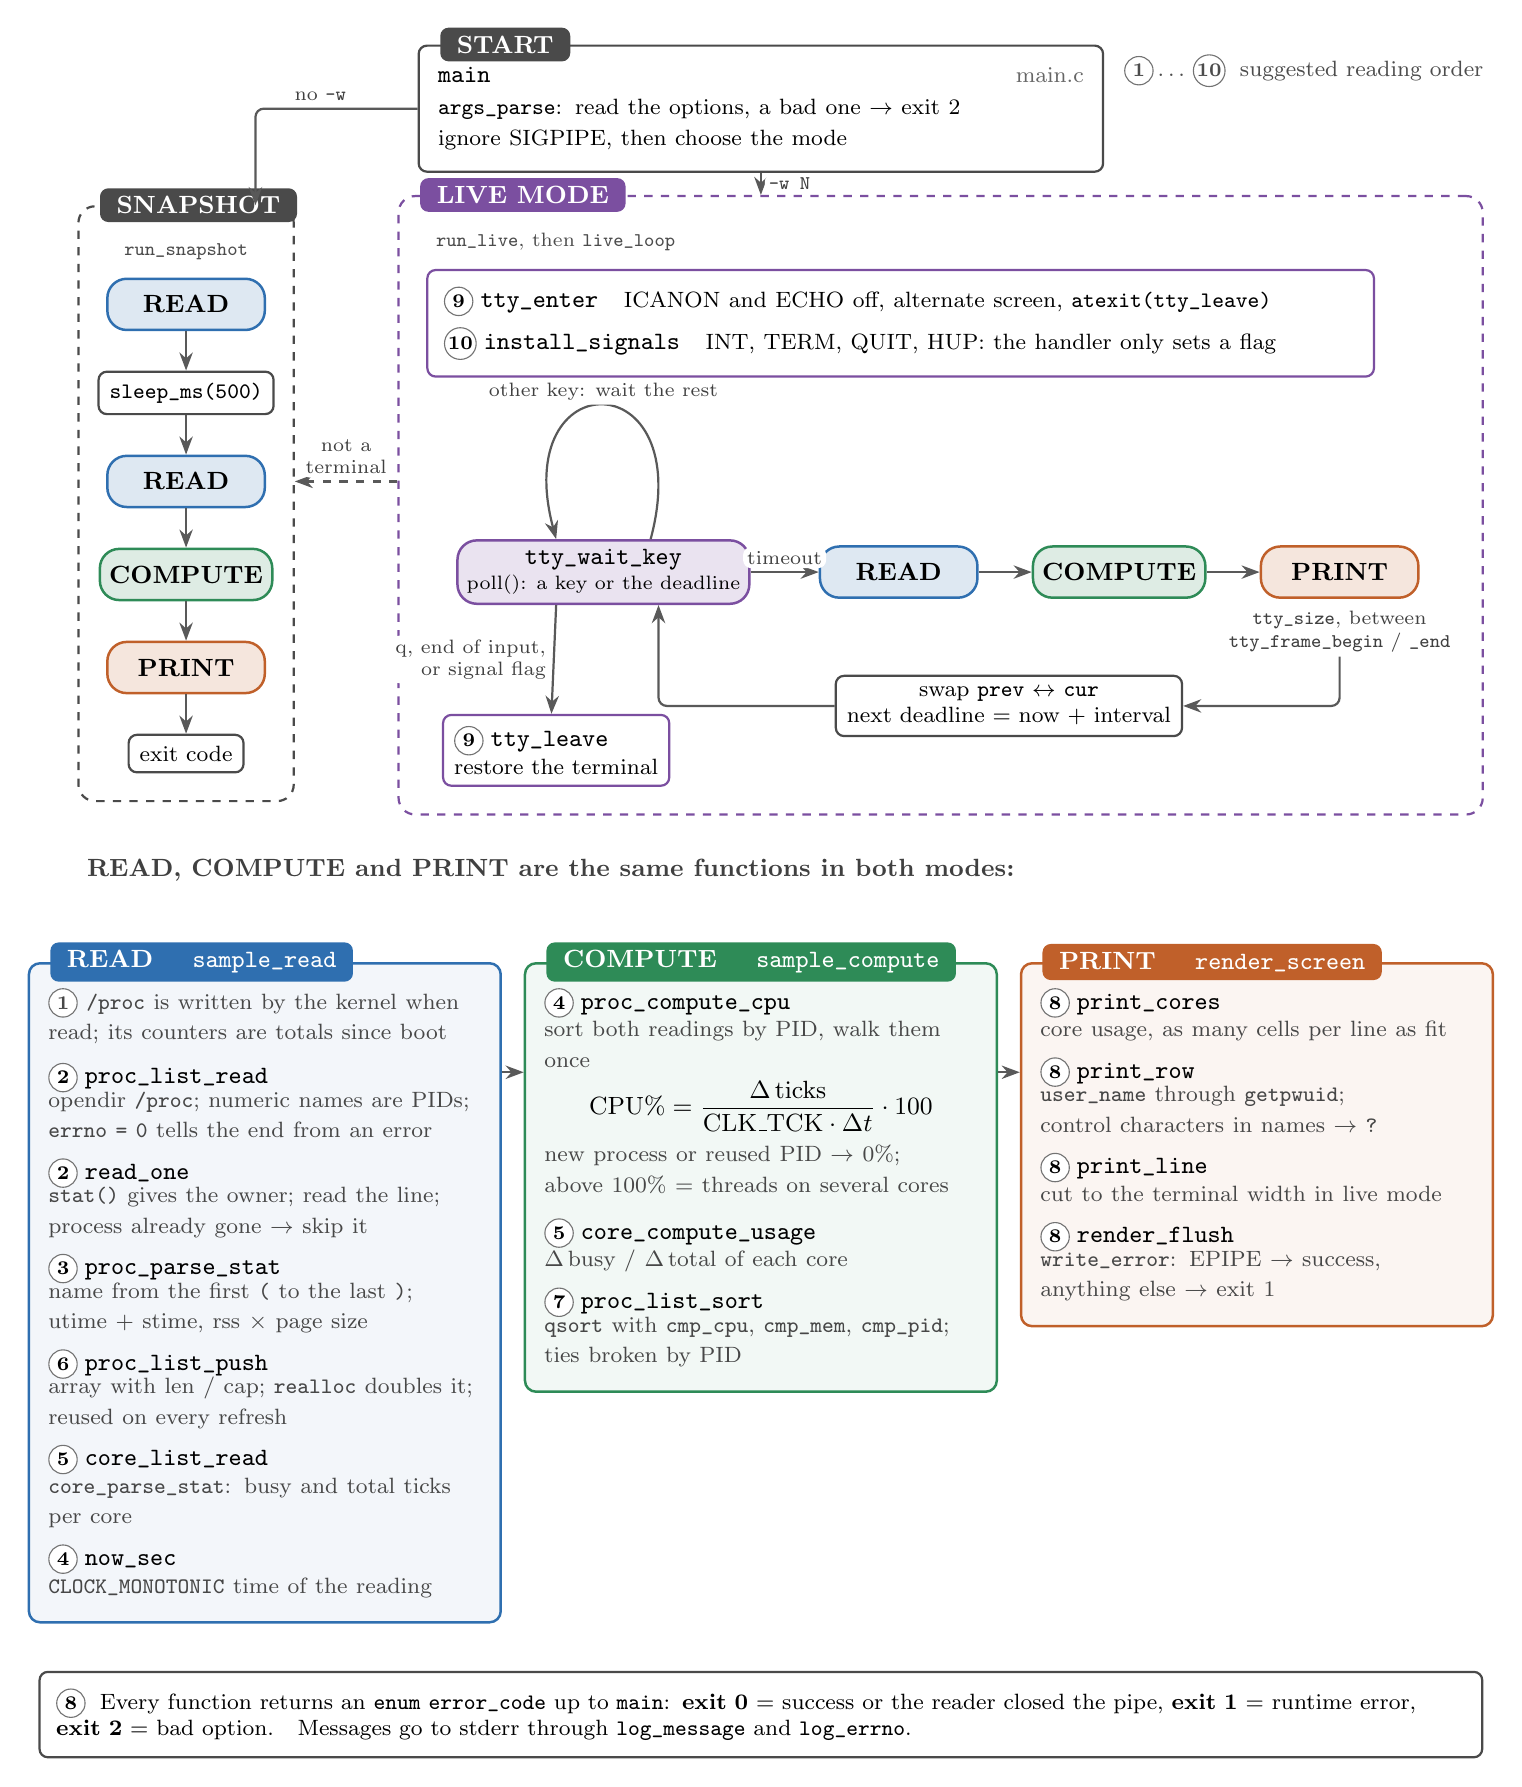
\begin{tikzpicture}

%% ---------- START ----------
\node[step=basec, text width=8.2cm, anchor=north, inner sep=7pt, inner ysep=8pt] (main) at (0,0) {%
  \textbf{\fn{main}}\hfill{\footnotesize\color{black!60}main.c}\\[2pt]
  {\footnotesize \fn{args_parse}: read the options, a bad one $\to$ exit 2\\
  ignore SIGPIPE, then choose the mode}};
\node[tab=basec] at ([xshift=8pt]main.north west) {START};
\node[font=\footnotesize, text=black!70, anchor=north east, align=right] at (9.3,0)
  {\st{1}\,\dots\,\st{10}\; suggested reading order};

%% ---------- SNAPSHOT ----------
\begin{scope}[node distance=5mm]
  \node[pill=readc] (s1) at (-7.3,-3.3) {READ};
  \node[step=basec, below=of s1, font=\footnotesize] (s2) {\fn{sleep_ms(500)}};
  \node[pill=readc, below=of s2] (s3) {READ};
  \node[pill=compc, below=of s3] (s4) {COMPUTE};
  \node[pill=printc, below=of s4] (s5) {PRINT};
  \node[step=basec, below=of s5, font=\footnotesize] (s6) {exit code};
\end{scope}
\foreach \a/\b in {s1/s2,s2/s3,s3/s4,s4/s5,s5/s6} \draw[flow] (\a) -- (\b);
\node[font=\scriptsize, text=black!70, align=center, above=1mm of s1] (snapfn) {\fn{run_snapshot}};
\begin{scope}[on background layer]
  \node[frame=basec, fit=(snapfn)(s1)(s6), inner xsep=10pt, inner ysep=10pt] (snapbox) {};
\end{scope}
\node[tab=basec] at ([xshift=8pt]snapbox.north west) {SNAPSHOT};

%% ---------- LIVE ----------
\node[step=ttyc, text width=11.6cm, anchor=north west, inner sep=6pt] (enter) at (-4.25,-2.85) {%
  \st{9}\;\textbf{\fn{tty_enter}}\quad{\footnotesize ICANON and ECHO off, alternate screen, \fn{atexit(tty_leave)}}\\[3pt]
  \st{10}\;\textbf{\fn{install_signals}}\quad{\footnotesize INT, TERM, QUIT, HUP: the handler only sets a flag}};

\node[pill=ttyc, minimum width=27mm] (wait) at (-2.0,-6.7)
  {\fn{tty_wait_key}\\[-2pt]{\scriptsize\mdseries poll(): a key or the deadline}};
\node[pill=readc] (lr) at (1.75,-6.7) {READ};
\node[pill=compc] (lc) at (4.55,-6.7) {COMPUTE};
\node[pill=printc] (lp) at (7.35,-6.7) {PRINT};
\node[lbl, below=1mm of lp, align=center] (fr) {\fn{tty_size}, between\\ \fn{tty_frame_begin} / \fn{_end}};
\node[step=basec, font=\footnotesize, align=center] (swap) at (3.15,-8.4)
  {swap \fn{prev} $\leftrightarrow$ \fn{cur}\\ next deadline = now + interval};
\node[step=ttyc, anchor=north] (leave) at (-2.6,-8.5)
  {\st{9}\;\textbf{\fn{tty_leave}}\\[-1pt]{\footnotesize restore the terminal}};

\draw[flow] (wait) -- node[lbl, above=1pt]{timeout} (lr);
\draw[flow] (lr) -- (lc);
\draw[flow] (lc) -- (lp);
\draw[flow] (fr.south) |- (swap.east);
\draw[flow] (swap.west) -| ([xshift=7mm]wait.south);
\draw[flow] ([xshift=-6mm]wait.south) -- node[lbl, left=1pt, align=right]{q, end of input,\\ or signal flag} ([xshift=-0.6mm]leave.north);
\draw[flow] ([xshift=6mm]wait.north) to[out=75, in=105, looseness=5]
  node[lbl, above=0pt, align=center]{other key: wait the rest} ([xshift=-6mm]wait.north);

\node[font=\scriptsize, text=black!70, anchor=south west] (livefn) at ([yshift=1mm]enter.north west) {\fn{run_live}, then \fn{live_loop}};
\begin{scope}[on background layer]
  \node[frame=ttyc, fit=(livefn)(enter)(fr)(swap)(leave), inner xsep=10pt, inner ysep=10pt] (livebox) {};
\end{scope}
\node[tab=ttyc] at ([xshift=8pt]livebox.north west) {LIVE MODE};

%% mode choice
\draw[flow] (main.west) -| node[lbl, pos=0.3, above=1pt]{no \fn{-w}} ([xshift=-5mm]snapbox.north east);
\draw[flow] (main.south) -- node[lbl, right=1pt]{\fn{-w N}} (main.south |- livebox.north);
\draw[flow, dashed] (livebox.west |- s3) -- node[lbl, above=1pt, align=center]{not a\\ terminal} (snapbox.east |- s3);

%% ---------- THE THREE STAGES ----------
\node[font=\small\bfseries, text=black!75, anchor=north west] (sharedcap) at ([yshift=-6mm]snapbox.south west)
  {READ, COMPUTE and PRINT are the same functions in both modes:};
\path let \p1 = ([yshift=-9mm]sharedcap.south) in coordinate (rowtop) at (0,\y1);

\node[stage=readc] (read) at ([xshift=-6.3cm]rowtop) {%
  {\footnotesize\color{black!72}\st{1} \fn{/proc} is written by the kernel when read;
   its counters are totals since boot}\\[5pt]
  \entry{2}{proc_list_read}{opendir \fn{/proc}; numeric names are PIDs;\\ \fn{errno = 0} tells the end from an error}
  \entry{2}{read_one}{\fn{stat()} gives the owner; read the line;\\ process already gone $\to$ skip it}
  \entry{3}{proc_parse_stat}{name from the first \fn{(} to the last \fn{)};\\ utime + stime, rss $\times$ page size}
  \entry{6}{proc_list_push}{array with len / cap; \fn{realloc} doubles it;\\ reused on every refresh}
  \entry{5}{core_list_read}{\fn{core_parse_stat}: busy and total ticks per core}
  \st{4}\;\textbf{\fn{now_sec}}\\[-1pt]{\footnotesize\color{black!72}\fn{CLOCK_MONOTONIC} time of the reading}};
\node[tab=readc] at ([xshift=8pt]read.north west) {READ \quad\mdseries\fn{sample_read}};

\node[stage=compc] (comp) at (rowtop) {%
  \entry{4}{proc_compute_cpu}{sort both readings by PID, walk them once}
  {\centering $\text{CPU\%} = \dfrac{\Delta\,\text{ticks}}{\text{CLK\_TCK}\cdot\Delta t}\cdot 100$\par}
  \vspace{4pt}
  {\footnotesize\color{black!72}new process or reused PID $\to$ 0\%;\\ above 100\% = threads on several cores}\\[6pt]
  \entry{5}{core_compute_usage}{$\Delta$\,busy / $\Delta$\,total of each core}
  \st{7}\;\textbf{\fn{proc_list_sort}}\\[-1pt]{\footnotesize\color{black!72}\fn{qsort} with \fn{cmp_cpu}, \fn{cmp_mem}, \fn{cmp_pid};\\ ties broken by PID}};
\node[tab=compc] at ([xshift=8pt]comp.north west) {COMPUTE \quad\mdseries\fn{sample_compute}};

\node[stage=printc] (print) at ([xshift=6.3cm]rowtop) {%
  \entry{8}{print_cores}{core usage, as many cells per line as fit}
  \entry{8}{print_row}{\fn{user_name} through \fn{getpwuid};\\ control characters in names $\to$ \fn{?}}
  \entry{8}{print_line}{cut to the terminal width in live mode}
  \st{8}\;\textbf{\fn{render_flush}}\\[-1pt]{\footnotesize\color{black!72}\fn{write_error}: EPIPE $\to$ success,\\ anything else $\to$ exit 1}};
\node[tab=printc] at ([xshift=8pt]print.north west) {PRINT \quad\mdseries\fn{render_screen}};

\coordinate (arrowy) at ([yshift=-1.4cm]rowtop);
\draw[flow] (read.east |- arrowy) -- (comp.west |- arrowy);
\draw[flow] (comp.east |- arrowy) -- (print.west |- arrowy);

%% ---------- ERRORS ----------
\node[step=basec, anchor=north, text width=17.9cm, inner sep=6pt, font=\footnotesize]
  (err) at ([yshift=-6mm]comp.south |- read.south) {%
  \st{8}\; Every function returns an \fn{enum error_code} up to \fn{main}:
  \textbf{exit 0} = success or the reader closed the pipe, \textbf{exit 1} = runtime error,
  \textbf{exit 2} = bad option.\quad Messages go to stderr through \fn{log_message} and \fn{log_errno}.};

\end{tikzpicture}

%% ====================================================================
%% Page 2: main and snapshot mode
%% ====================================================================
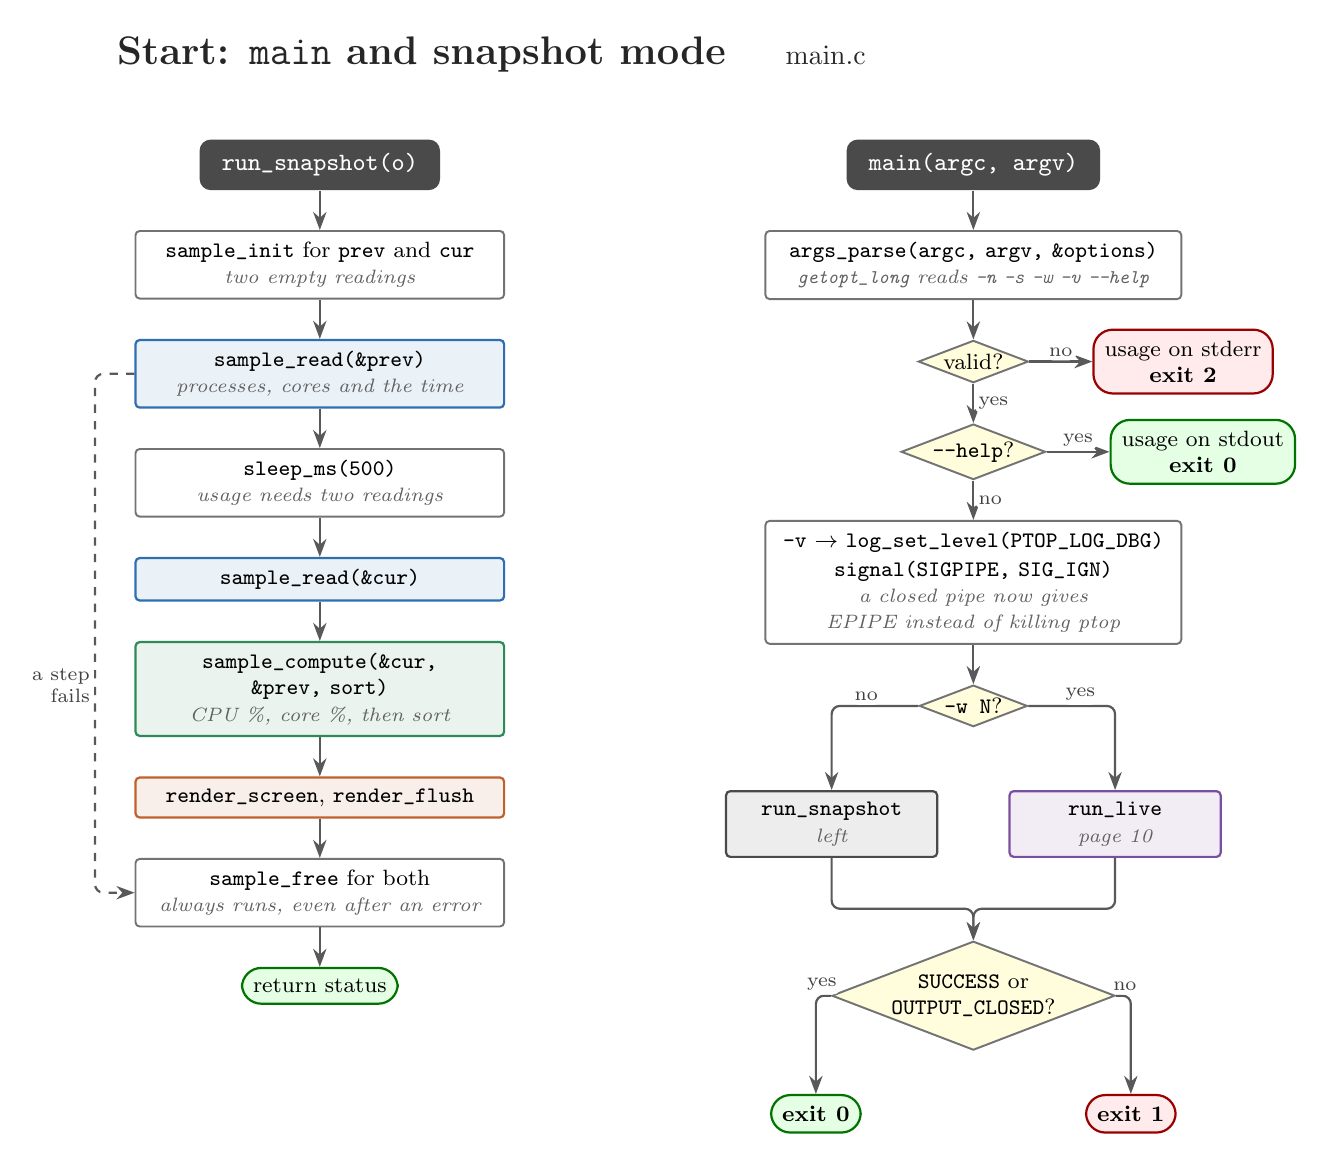
\begin{tikzpicture}[node distance=5mm and 8mm]
\node[pagehead] at (-11,1.4) {Start: \fn{main} and snapshot mode \quad{\normalsize\mdseries main.c}};

%% main
\node[ftitle=basec] (t) at (0,0) {\fn{main(argc, argv)}};
\node[act, below=of t] (a1) {\fn{args_parse(argc, argv, &options)}\\\nt{\fn{getopt_long} reads \texttt{-n -s -w -v -{}-help}}};
\node[ask, below=of a1] (q1) {valid?};
\node[bad, right=of q1] (r1) {usage on stderr\\\textbf{exit 2}};
\node[ask, below=of q1] (q2) {\texttt{-{}-help}?};
\node[good, right=of q2] (r2) {usage on stdout\\\textbf{exit 0}};
\node[act, below=of q2] (a2) {\fn{-v} $\to$ \fn{log_set_level(PTOP_LOG_DBG)}\\[1pt]\fn{signal(SIGPIPE, SIG_IGN)}\\\nt{a closed pipe now gives EPIPE instead of killing ptop}};
\node[ask, below=of a2] (q3) {\fn{-w N}?};
\node[call=basec, text width=2.4cm] (m1) at ([xshift=-18mm,yshift=-15mm]q3) {\fn{run_snapshot}\\\nt{left}};
\node[call=ttyc, text width=2.4cm] (m2) at ([xshift=18mm,yshift=-15mm]q3) {\fn{run_live}\\\nt{page 10}};
\node[ask, below=27mm of q3] (q4) {\fn{SUCCESS} or\\\fn{OUTPUT_CLOSED}?};
\node[good] (e0) at ([xshift=-20mm,yshift=-15mm]q4) {\textbf{exit 0}};
\node[bad] (e1) at ([xshift=20mm,yshift=-15mm]q4) {\textbf{exit 1}};

\draw[flow] (t) -- (a1);
\draw[flow] (a1) -- (q1);
\draw[flow] (q1) -- node[lbl,above]{no} (r1);
\draw[flow] (q1) -- node[lbl,right]{yes} (q2);
\draw[flow] (q2) -- node[lbl,above]{yes} (r2);
\draw[flow] (q2) -- node[lbl,right]{no} (a2);
\draw[flow] (a2) -- (q3);
\draw[flow] (q3.west) -| node[lbl,pos=0.3,above]{no} (m1.north);
\draw[flow] (q3.east) -| node[lbl,pos=0.3,above]{yes} (m2.north);
\draw[flow] (m1.south) |- ([yshift=4mm]q4.north) -- (q4.north);
\draw[flow] (m2.south) |- ([yshift=4mm]q4.north) -- (q4.north);
\draw[flow] (q4.west) -| node[lbl,pos=0.3,above]{yes} (e0.north);
\draw[flow] (q4.east) -| node[lbl,pos=0.3,above]{no} (e1.north);

%% run_snapshot
\node[ftitle=basec] (st) at (-8.3,0) {\fn{run_snapshot(o)}};
\begin{scope}[act/.append style={text width=4.4cm}]
\node[act, below=of st] (b1) {\fn{sample_init} for \fn{prev} and \fn{cur}\\\nt{two empty readings}};
\node[call=readc, below=of b1] (b2) {\fn{sample_read(&prev)}\\\nt{processes, cores and the time}};
\node[act, below=of b2] (b3) {\fn{sleep_ms(500)}\\\nt{usage needs two readings}};
\node[call=readc, below=of b3] (b4) {\fn{sample_read(&cur)}};
\node[call=compc, below=of b4] (b5) {\fn{sample_compute(&cur, &prev, sort)}\\\nt{CPU \%, core \%, then sort}};
\node[call=printc, below=of b5] (b6) {\fn{render_screen}, \fn{render_flush}};
\node[act, below=of b6] (b7) {\fn{sample_free} for both\\\nt{always runs, even after an error}};
\end{scope}
\node[good, below=of b7] (b8) {return status};
\foreach \a/\b in {st/b1,b1/b2,b2/b3,b3/b4,b4/b5,b5/b6,b6/b7,b7/b8} \draw[flow] (\a) -- (\b);
\draw[flow, dashed] (b2.west) -- ++(-5mm,0) |- node[lbl, pos=0.3, left, align=right]{a step\\fails} (b7.west);
\end{tikzpicture}

%% ====================================================================
%% Page 3: proc_list_read and read_one
%% ====================================================================
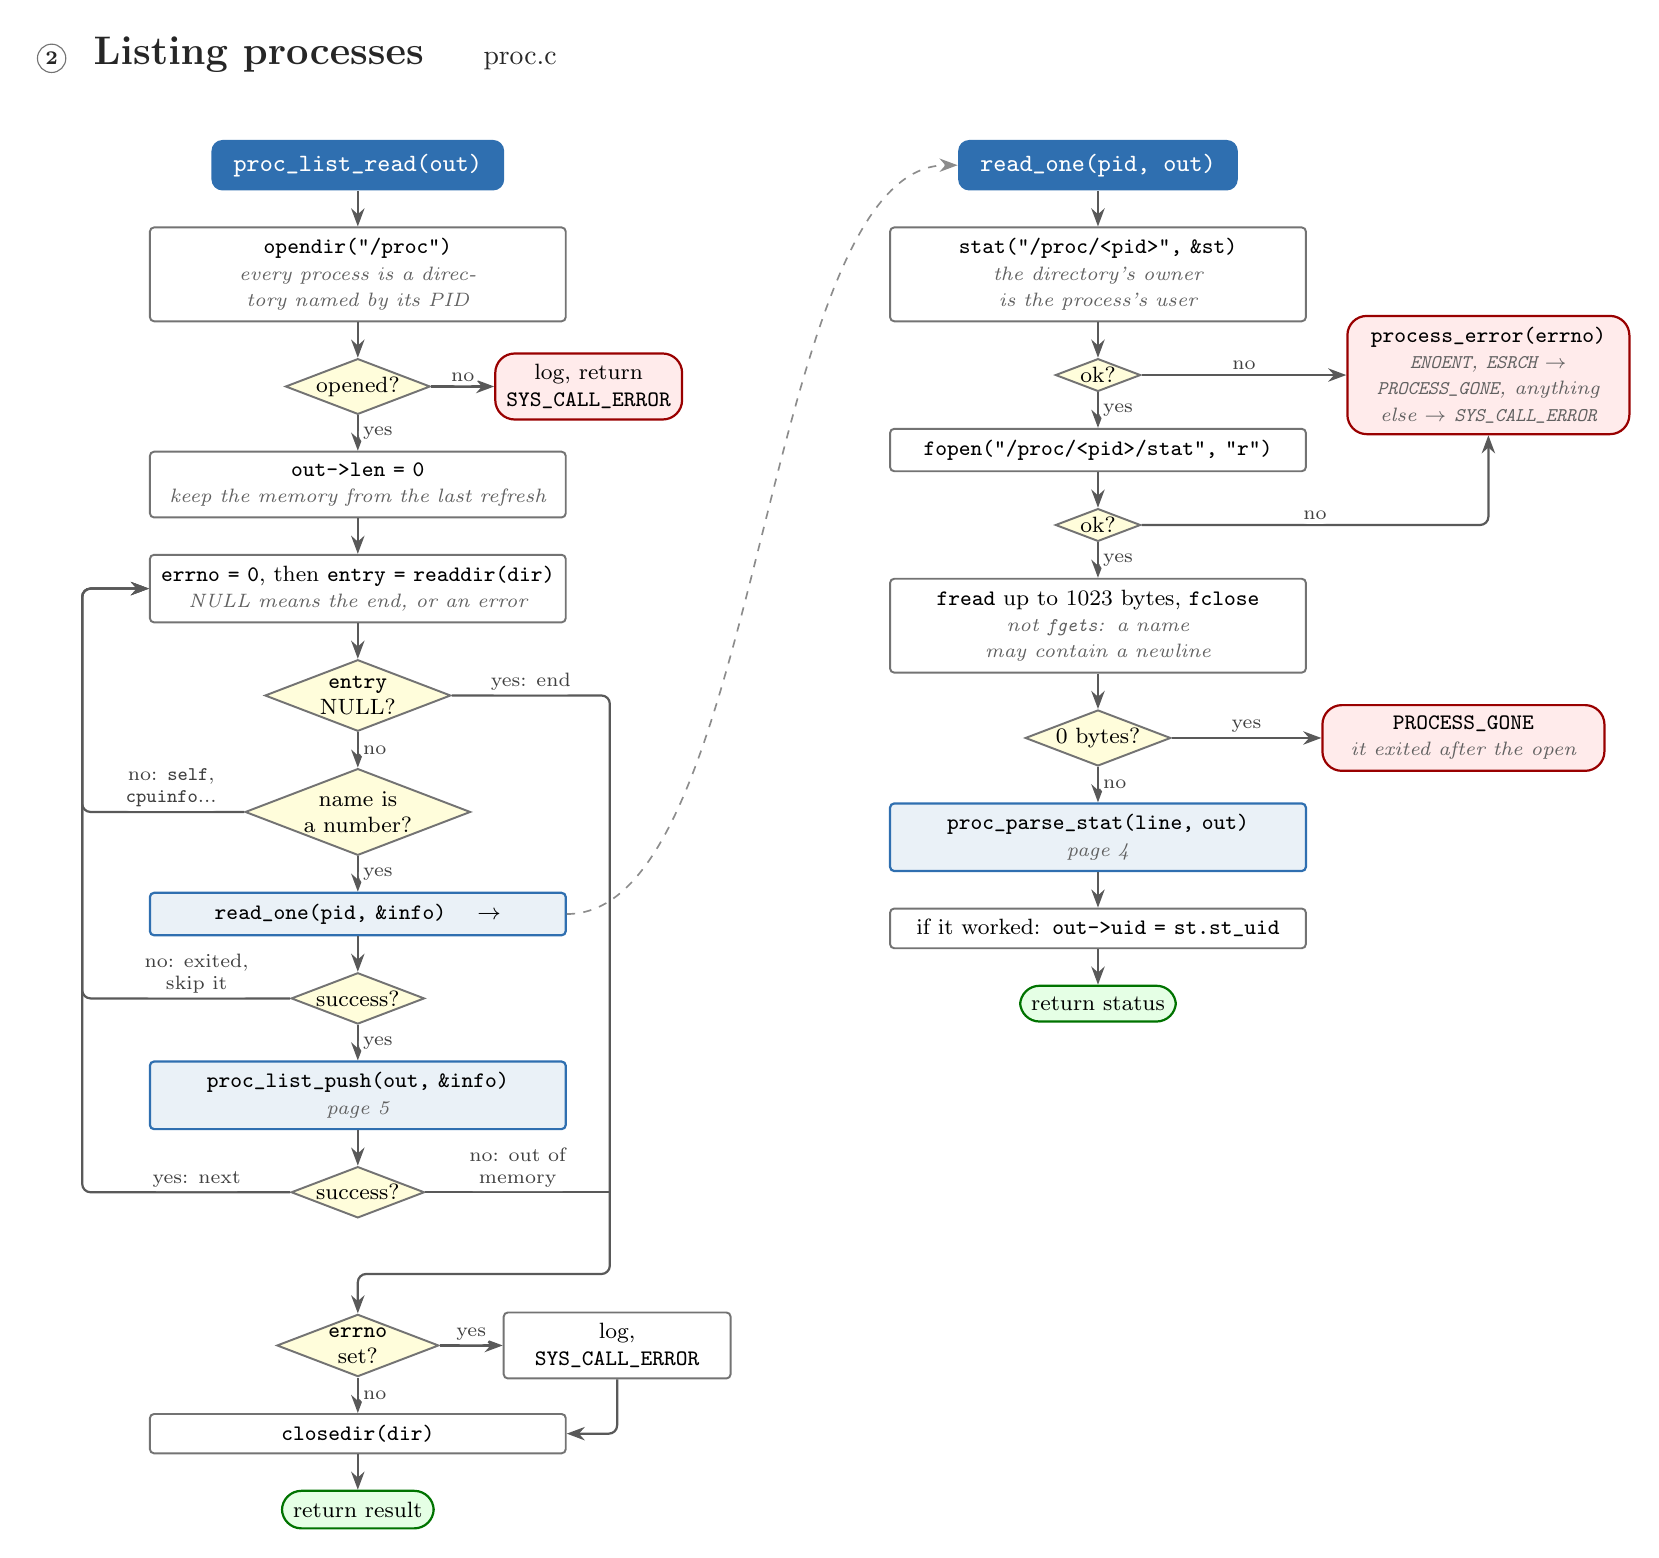
\begin{tikzpicture}[node distance=4.5mm and 8mm]
\node[pagehead] at (-4.2,1.4) {\st{2}\; Listing processes \quad{\normalsize\mdseries proc.c}};
\coordinate (L) at (-3.5,0);
\coordinate (R) at (3.2,0);

\node[ftitle=readc] (t) at (0,0) {\fn{proc_list_read(out)}};
\node[act, below=of t] (n1) {\fn{opendir("/proc")}\\\nt{every process is a directory named by its PID}};
\node[ask, below=of n1] (q1) {opened?};
\node[bad, right=of q1] (r1) {log, return\\\fn{SYS_CALL_ERROR}};
\node[act, below=of q1] (n2) {\fn{out->len = 0}\\\nt{keep the memory from the last refresh}};
\node[act, below=of n2] (n3) {\fn{errno = 0}, then \fn{entry = readdir(dir)}\\\nt{NULL means the end, or an error}};
\node[ask, below=of n3] (q2) {\fn{entry}\\NULL?};
\node[ask, below=of q2] (q3) {name is\\a number?};
\node[call=readc, below=of q3] (n4) {\fn{read_one(pid, &info)} \quad$\to$};
\node[ask, below=of n4] (q4) {success?};
\node[call=readc, below=of q4] (n5) {\fn{proc_list_push(out, &info)}\\\nt{page 5}};
\node[ask, below=of n5] (q5) {success?};
\node[ask, below=12mm of q5] (q6) {\fn{errno}\\set?};
\node[act, right=of q6, text width=2.6cm] (r6) {log,\\\fn{SYS_CALL_ERROR}};
\node[act, below=of q6] (n6) {\fn{closedir(dir)}};
\node[good, below=of n6] (r) {return result};

\draw[flow] (t) -- (n1);
\draw[flow] (n1) -- (q1);
\draw[flow] (q1) -- node[lbl,above]{no} (r1);
\draw[flow] (q1) -- node[lbl,right]{yes} (n2);
\draw[flow] (n2) -- (n3);
\draw[flow] (n3) -- (q2);
\draw[flow] (q2) -- node[lbl,right]{no} (q3);
\draw[flow] (q3) -- node[lbl,right]{yes} (n4);
\draw[flow] (n4) -- (q4);
\draw[flow] (q4) -- node[lbl,right]{yes} (n5);
\draw[flow] (n5) -- (q5);
\draw[flow] (q3.west) -- node[lbl,above,pos=0.45,align=center]{no: \fn{self},\\\fn{cpuinfo}...} (q3.west -| L) |- (n3.west);
\draw[flow] (q4.west) -- node[lbl,above,pos=0.45,align=center]{no: exited,\\skip it} (q4.west -| L) |- (n3.west);
\draw[flow] (q5.west) -- node[lbl,above,pos=0.45]{yes: next} (q5.west -| L) |- (n3.west);
\draw[flow] (q2.east) -- node[lbl,above,pos=0.5]{yes: end} (q2.east -| R) |- ([yshift=5mm]q6.north) -- (q6.north);
\draw[flow, -] (q5.east) -- node[lbl,above,pos=0.5,align=center]{no: out of\\memory} (q5.east -| R);
\draw[flow] (q6) -- node[lbl,above]{yes} (r6);
\draw[flow] (q6) -- node[lbl,right]{no} (n6);
\draw[flow] (r6.south) |- (n6.east);
\draw[flow] (n6) -- (r);

%% read_one
\node[ftitle=readc] (u) at (9.4,0) {\fn{read_one(pid, out)}};
\node[act, below=of u] (o1) {\fn{stat("/proc/<pid>", &st)}\\\nt{the directory's owner is the process's user}};
\node[ask, below=of o1] (p1) {ok?};
\node[act, below=of p1] (o2) {\fn{fopen("/proc/<pid>/stat", "r")}};
\node[ask, below=of o2] (p2) {ok?};
\node[act, below=of p2] (o3) {\fn{fread} up to 1023 bytes, \fn{fclose}\\\nt{not \fn{fgets}: a name may contain a newline}};
\node[ask, below=of o3] (p3) {0 bytes?};
\node[call=readc, below=of p3] (o4) {\fn{proc_parse_stat(line, out)}\\\nt{page 4}};
\node[act, below=of o4] (o5) {if it worked: \fn{out->uid = st.st_uid}};
\node[good, below=of o5] (u9) {return status};
\node[bad, right=26mm of p1, text width=3.3cm] (x1) {\fn{process_error(errno)}\\\nt{\fn{ENOENT}, \fn{ESRCH} $\to$ \fn{PROCESS_GONE}, anything else $\to$ \fn{SYS_CALL_ERROR}}};
\node[bad, right=19mm of p3, text width=3.3cm] (x3) {\fn{PROCESS_GONE}\\\nt{it exited after the open}};

\draw[flow] (u) -- (o1);
\draw[flow] (o1) -- (p1);
\draw[flow] (p1) -- node[lbl,right]{yes} (o2);
\draw[flow] (o2) -- (p2);
\draw[flow] (p2) -- node[lbl,right]{yes} (o3);
\draw[flow] (o3) -- (p3);
\draw[flow] (p3) -- node[lbl,right]{no} (o4);
\draw[flow] (o4) -- (o5);
\draw[flow] (o5) -- (u9);
\draw[flow] (p1) -- node[lbl,above]{no} (x1);
\draw[flow] (p2.east) -| node[lbl,pos=0.25,above]{no} (x1.south);
\draw[flow] (p3) -- node[lbl,above]{yes} (x3);
\draw[black!45, dashed, ->, line width=0.6pt] (n4.east) .. controls +(2.5,0) and +(-2.5,0) .. (u.west);
\end{tikzpicture}

%% ====================================================================
%% Page 4: proc_parse_stat
%% ====================================================================
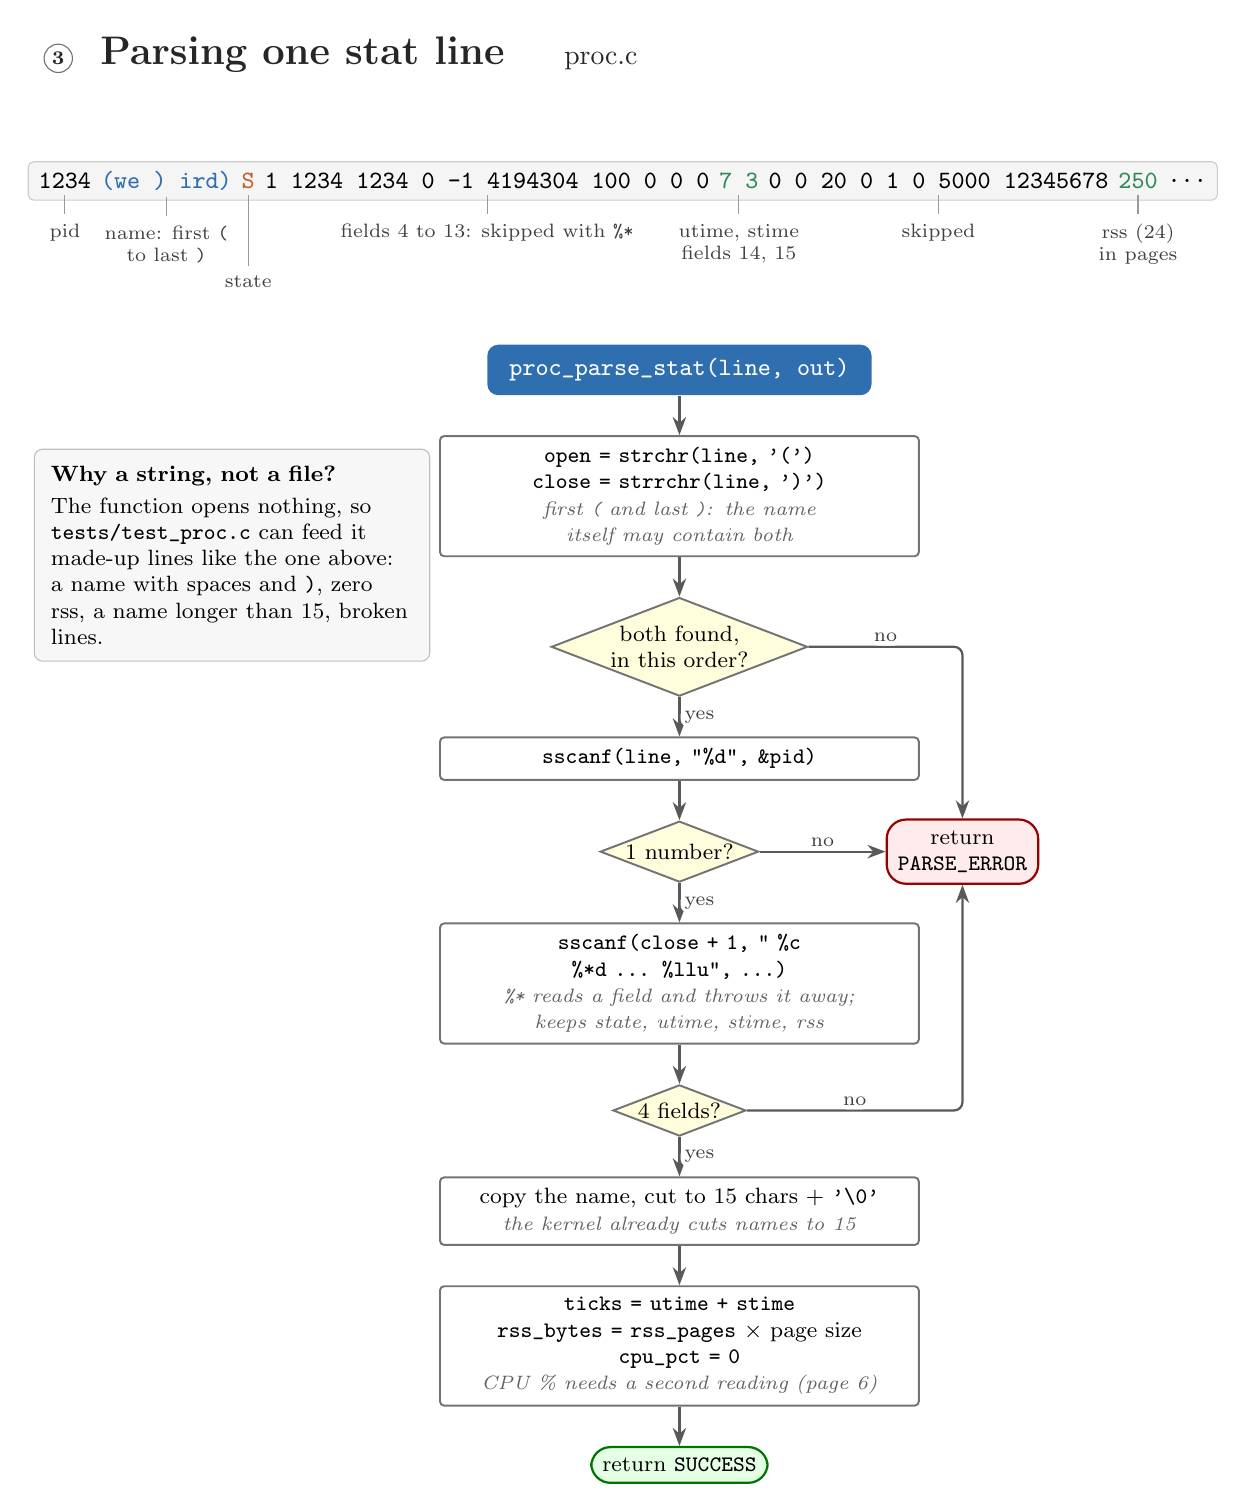
\begin{tikzpicture}[node distance=5mm and 8mm]
\node[pagehead] at (-8.2,1.6) {\st{3}\; Parsing one stat line \quad{\normalsize\mdseries proc.c}};

% the example line from tests/test_proc.c
\node[ex, anchor=west] (e1) at (-8.2,0) {1234};
\node[ex, right=0pt of e1, text=readc, font=\ttfamily\small\bfseries] (e2) {(we ) ird)};
\node[ex, right=0pt of e2, text=printc, font=\ttfamily\small\bfseries] (e3) {S};
\node[ex, right=0pt of e3] (e4) {1 1234 1234 0 -1 4194304 100 0 0 0};
\node[ex, right=0pt of e4, text=compc, font=\ttfamily\small\bfseries] (e5) {7 3};
\node[ex, right=0pt of e5] (e6) {0 0 20 0 1 0 5000 12345678};
\node[ex, right=0pt of e6, text=compc, font=\ttfamily\small\bfseries] (e7) {250};
\node[ex, right=0pt of e7] (e8) {...};
\begin{scope}[on background layer]
  \node[fill=black!4, draw=black!20, rounded corners=2pt, fit=(e1)(e8), inner sep=2pt] {};
\end{scope}
\draw[black!40] (e1.south) -- ++(0,-2.5mm) node[exl]{pid};
\draw[black!40] (e2.south) -- ++(0,-2.5mm) node[exl]{name: first \fn{(}\\to last \fn{)}};
\draw[black!40] (e3.south) -- ++(0,-9mm) node[exl]{state};
\draw[black!40] (e4.south) -- ++(0,-2.5mm) node[exl]{fields 4 to 13: skipped with \texttt{\%*}};
\draw[black!40] (e5.south) -- ++(0,-2.5mm) node[exl]{utime, stime\\fields 14, 15};
\draw[black!40] (e6.south) -- ++(0,-2.5mm) node[exl]{skipped};
\draw[black!40] (e7.south) -- ++(0,-2.5mm) node[exl]{rss (24)\\in pages};

\node[ftitle=readc] (t) at (0,-2.4) {\fn{proc_parse_stat(line, out)}};
\begin{scope}[act/.append style={text width=5.8cm}]
\node[act, below=of t] (a1) {\fn{open = strchr(line, '(')}\\\fn{close = strrchr(line, ')')}\\\nt{first \fn{(} and last \fn{)}: the name itself may contain both}};
\node[ask, below=of a1] (q1) {both found,\\in this order?};
\node[act, below=of q1] (a2) {\texttt{sscanf(line, "\%d", \&pid)}};
\node[ask, below=of a2] (q2) {1 number?};
\node[act, below=of q2] (a3) {\texttt{sscanf(close + 1, " \%c \%*d ... \%llu", ...)}\\\nt{\texttt{\%*} reads a field and throws it away; keeps state, utime, stime, rss}};
\node[ask, below=of a3] (q3) {4 fields?};
\node[act, below=of q3] (a4) {copy the name, cut to 15 chars + \fn{'\0'}\\\nt{the kernel already cuts names to 15}};
\node[act, below=of a4] (a5) {\fn{ticks = utime + stime}\\\fn{rss_bytes = rss_pages} $\times$ page size\\\fn{cpu_pct = 0}\\\nt{CPU \% needs a second reading (page 6)}};
\end{scope}
\node[good, below=of a5] (r) {return \fn{SUCCESS}};
\node[bad, right=16mm of q2] (x) {return\\\fn{PARSE_ERROR}};

\foreach \a/\b in {t/a1,a1/q1,a2/q2,a3/q3,a4/a5,a5/r} \draw[flow] (\a) -- (\b);
\draw[flow] (q1) -- node[lbl,right]{yes} (a2);
\draw[flow] (q2) -- node[lbl,right]{yes} (a3);
\draw[flow] (q3) -- node[lbl,right]{yes} (a4);
\draw[flow] (q1.east) -| node[lbl,pos=0.25,above]{no} (x.north);
\draw[flow] (q2) -- node[lbl,above]{no} (x);
\draw[flow] (q3.east) -| node[lbl,pos=0.25,above]{no} (x.south);

\node[side=4.6cm, anchor=north west] at (-8.2,-3.4) {%
  \textbf{Why a string, not a file?}\\[2pt]
  The function opens nothing, so \fn{tests/test_proc.c} can feed it made-up lines like the one above:
  a name with spaces and \fn{)}, zero rss, a name longer than 15, broken lines.};
\end{tikzpicture}

%% ====================================================================
%% Page 5: proc_list_push and the list's life
%% ====================================================================
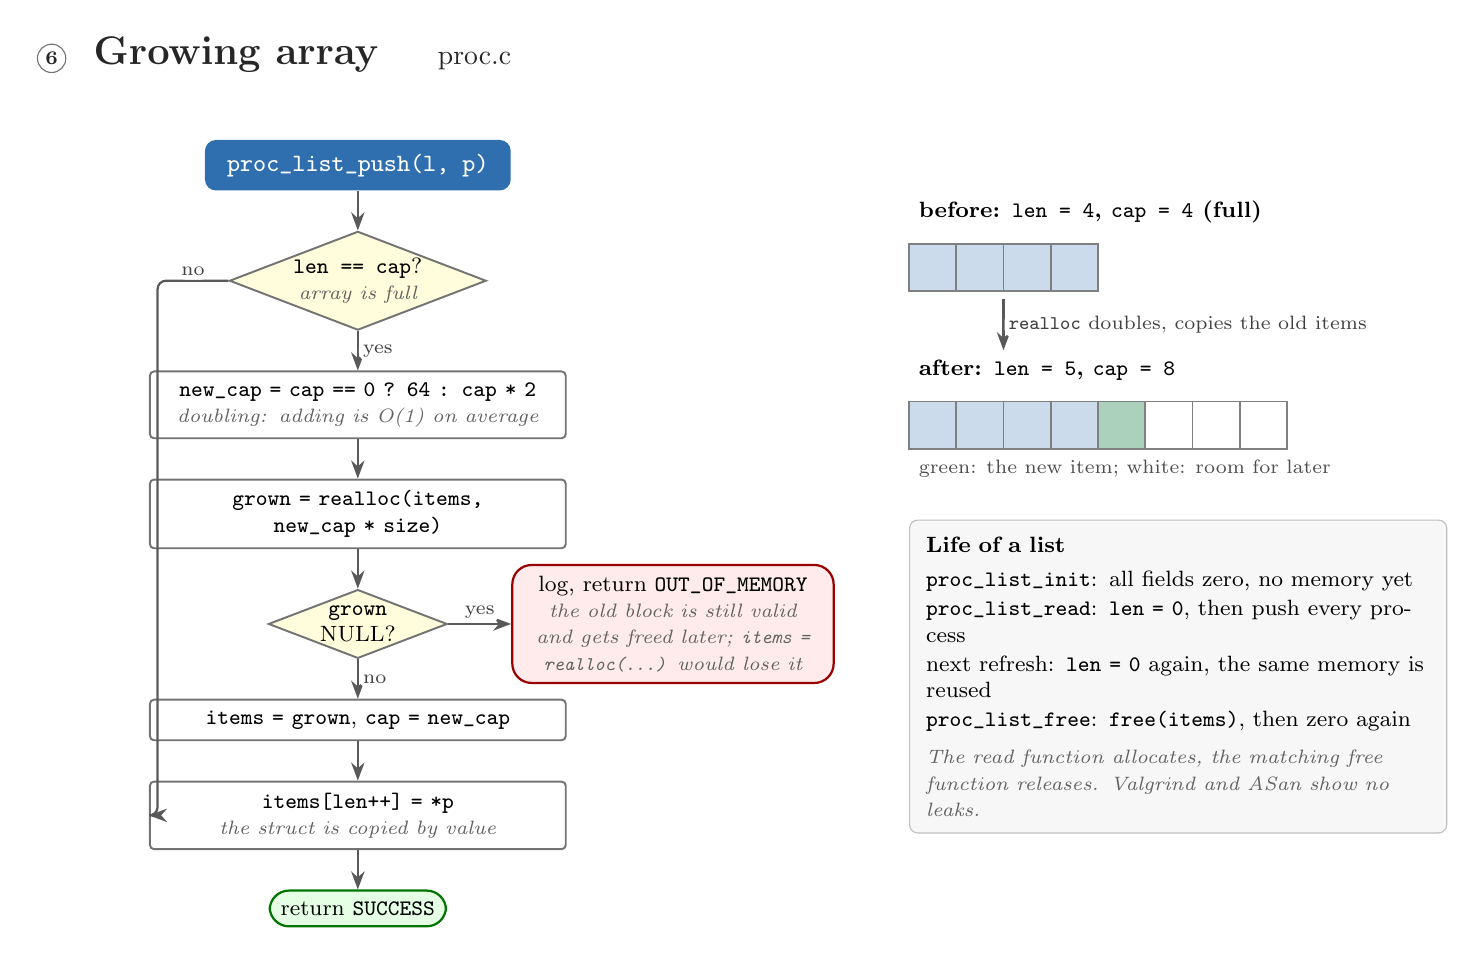
\begin{tikzpicture}[node distance=5mm and 8mm]
\node[pagehead] at (-4.2,1.4) {\st{6}\; Growing array \quad{\normalsize\mdseries proc.c}};

\node[ftitle=readc] (t) at (0,0) {\fn{proc_list_push(l, p)}};
\node[ask, below=of t] (q1) {\fn{len == cap}?\\\nt{array is full}};
\node[act, below=of q1] (a1) {\fn{new_cap = cap == 0 ? 64 : cap * 2}\\\nt{doubling: adding is O(1) on average}};
\node[act, below=of a1] (a2) {\fn{grown = realloc(items, new_cap * size)}};
\node[ask, below=of a2] (q2) {\fn{grown}\\NULL?};
\node[act, below=of q2] (a3) {\fn{items = grown}, \fn{cap = new_cap}};
\node[act, below=of a3] (a4) {\fn{items[len++] = *p}\\\nt{the struct is copied by value}};
\node[good, below=of a4] (r) {return \fn{SUCCESS}};
\node[bad, right=of q2, text width=3.8cm] (x) {log, return \fn{OUT_OF_MEMORY}\\\nt{the old block is still valid and gets freed later; \fn{items = realloc(...)} would lose it}};

\foreach \a/\b in {t/q1,a1/a2,a2/q2,a3/a4,a4/r} \draw[flow] (\a) -- (\b);
\draw[flow] (q1) -- node[lbl,right]{yes} (a1);
\draw[flow] (q2) -- node[lbl,right]{no} (a3);
\draw[flow] (q2) -- node[lbl,above]{yes} (x);
\draw[flow] (q1.west) -- node[lbl,above]{no} ++(-9mm,0) |- (a4.west);

% picture of the array
\node[font=\footnotesize\bfseries, anchor=west] at (7.0,-0.6) {before: \fn{len = 4}, \fn{cap = 4} (full)};
\foreach \i in {0,...,3} \node[cell, fill=readc!25] at (7.3+\i*0.6,-1.3) {};
\node[font=\footnotesize\bfseries, anchor=west] at (7.0,-2.6) {after: \fn{len = 5}, \fn{cap = 8}};
\foreach \i in {0,...,3} \node[cell, fill=readc!25] at (7.3+\i*0.6,-3.3) {};
\node[cell, fill=compc!40] at (7.3+4*0.6,-3.3) {};
\foreach \i in {5,...,7} \node[cell, fill=white] at (7.3+\i*0.6,-3.3) {};
\draw[flow] (8.2,-1.7) -- node[lbl,right]{\fn{realloc} doubles, copies the old items} (8.2,-2.35);
\node[font=\scriptsize, text=black!70, anchor=west] at (7.0,-3.85) {green: the new item; white: room for later};

\node[side=6.4cm, anchor=north west] at (7.0,-4.5) {%
  \textbf{Life of a list}\\[3pt]
  \fn{proc_list_init}: all fields zero, no memory yet\\[1pt]
  \fn{proc_list_read}: \fn{len = 0}, then push every process\\[1pt]
  next refresh: \fn{len = 0} again, the same memory is reused\\[1pt]
  \fn{proc_list_free}: \fn{free(items)}, then zero again\\[4pt]
  \nt{The read function allocates, the matching free function releases. Valgrind and ASan show no leaks.}};
\end{tikzpicture}

%% ====================================================================
%% Page 6: proc_compute_cpu
%% ====================================================================
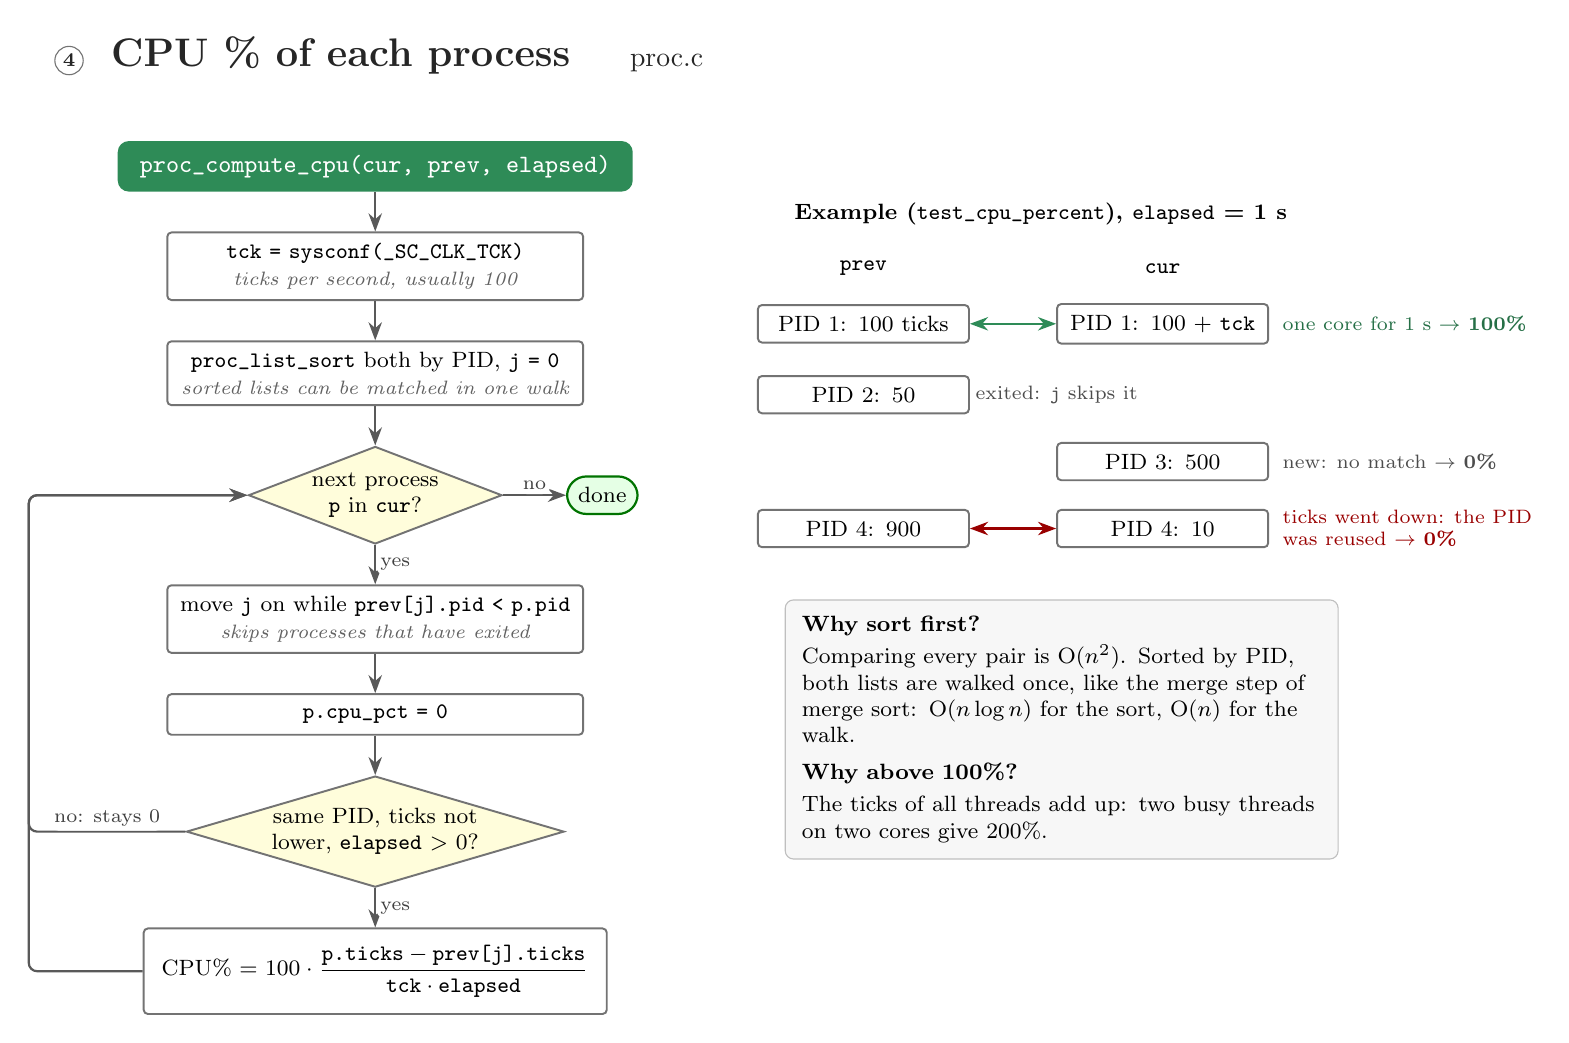
\begin{tikzpicture}[node distance=5mm and 8mm]
\node[pagehead] at (-4.2,1.4) {\st{4}\; CPU \% of each process \quad{\normalsize\mdseries proc.c}};
\coordinate (L) at (-4.4,0);

\node[ftitle=compc] (t) at (0,0) {\fn{proc_compute_cpu(cur, prev, elapsed)}};
\node[act, below=of t] (a1) {\fn{tck = sysconf(_SC_CLK_TCK)}\\\nt{ticks per second, usually 100}};
\node[act, below=of a1] (a2) {\fn{proc_list_sort} both by PID, \fn{j = 0}\\\nt{sorted lists can be matched in one walk}};
\node[ask, below=of a2] (q1) {next process\\\fn{p} in \fn{cur}?};
\node[good, right=of q1] (r) {done};
\node[act, below=of q1] (a3) {move \fn{j} on while \fn{prev[j].pid < p.pid}\\\nt{skips processes that have exited}};
\node[act, below=of a3] (a4) {\fn{p.cpu_pct = 0}};
\node[ask, below=of a4, aspect=3.4] (q2) {same PID, ticks not\\lower, \fn{elapsed} $>$ 0?};
\node[act, below=of q2, text width=5.6cm, inner ysep=6pt] (a5)
  {$\text{CPU\%} = 100\cdot\dfrac{\fn{p.ticks} - \fn{prev[j].ticks}}{\fn{tck}\cdot\fn{elapsed}}$};

\foreach \a/\b in {t/a1,a1/a2,a2/q1,a3/a4,a4/q2} \draw[flow] (\a) -- (\b);
\draw[flow] (q1) -- node[lbl,right]{yes} (a3);
\draw[flow] (q1) -- node[lbl,above]{no} (r);
\draw[flow] (q2) -- node[lbl,right]{yes} (a5);
\draw[flow] (q2.west) -- node[lbl,above,pos=0.5,align=center]{no: stays 0} (q2.west -| L) |- (q1.west);
\draw[flow] (a5.west) -- (a5.west -| L) |- (q1.west);

% example from test_cpu_percent
\node[font=\footnotesize\bfseries, anchor=west] at (5.2,-0.6) {Example (\fn{test_cpu_percent}), \fn{elapsed} = 1 s};
\node[font=\footnotesize\bfseries] at (6.2,-1.3) {\fn{prev}};
\node[font=\footnotesize\bfseries] at (10.0,-1.3) {\fn{cur}};
\node[act, text width=2.4cm] (p1) at (6.2,-2.0) {PID 1: 100 ticks};
\node[act, text width=2.4cm] (p2) at (6.2,-2.9) {PID 2: 50};
\node[act, text width=2.4cm] (p4) at (6.2,-4.6) {PID 4: 900};
\node[act, text width=2.4cm] (c1) at (10.0,-2.0) {PID 1: 100 + \fn{tck}};
\node[act, text width=2.4cm] (c3) at (10.0,-3.75) {PID 3: 500};
\node[act, text width=2.4cm] (c4) at (10.0,-4.6) {PID 4: 10};
\draw[<->, line width=0.8pt, compc] (p1) -- (c1);
\draw[<->, line width=0.8pt, red!60!black] (p4) -- (c4);
\node[font=\scriptsize, anchor=west, text=compc!80!black] at (11.4,-2.0) {one core for 1 s $\to$ \textbf{100\%}};
\node[font=\scriptsize, anchor=west, text=black!70] at (7.5,-2.9) {exited: \fn{j} skips it};
\node[font=\scriptsize, anchor=west, text=black!70] at (11.4,-3.75) {new: no match $\to$ \textbf{0\%}};
\node[font=\scriptsize, anchor=west, text=red!60!black, align=left] at (11.4,-4.6) {ticks went down: the PID\\was reused $\to$ \textbf{0\%}};

\node[side=6.6cm, anchor=north west] at (5.2,-5.5) {%
  \textbf{Why sort first?}\\[2pt]
  Comparing every pair is O($n^2$). Sorted by PID, both lists are walked once,
  like the merge step of merge sort: O($n \log n$) for the sort, O($n$) for the walk.\\[4pt]
  \textbf{Why above 100\%?}\\[2pt]
  The ticks of all threads add up: two busy threads on two cores give 200\%.};
\end{tikzpicture}

%% ====================================================================
%% Page 7: core usage
%% ====================================================================
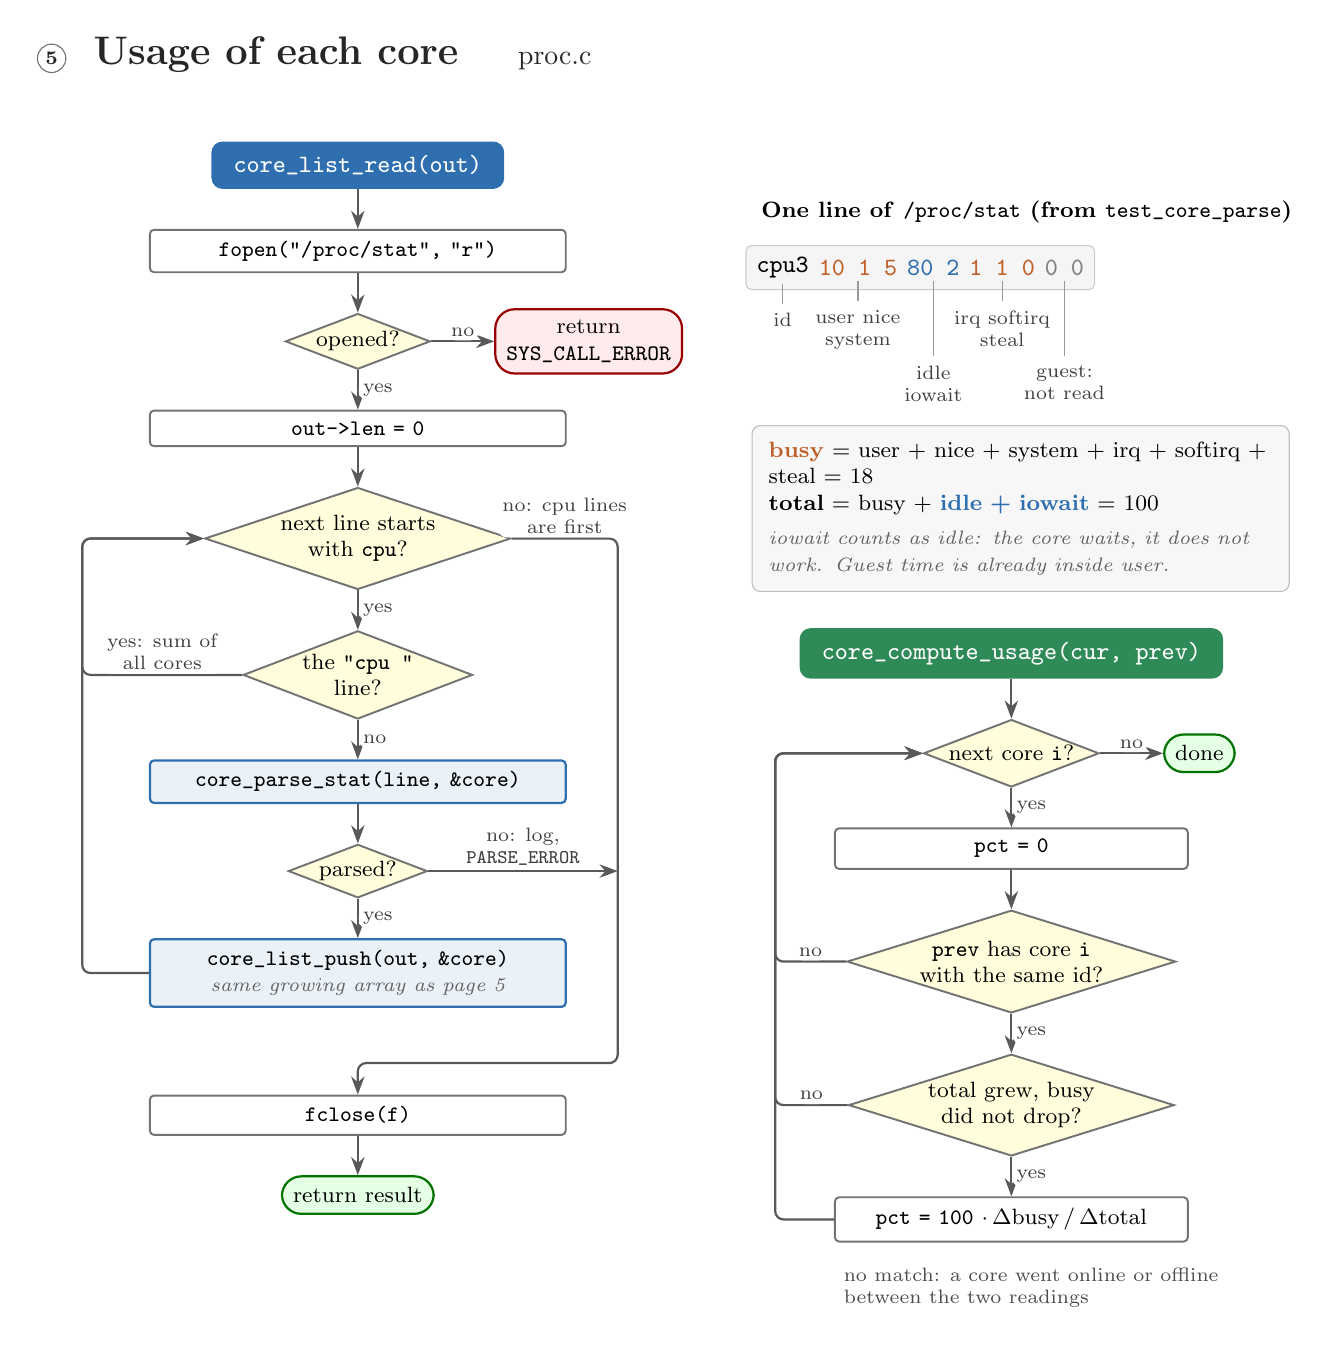
\begin{tikzpicture}[node distance=5mm and 8mm]
\node[pagehead] at (-4.2,1.4) {\st{5}\; Usage of each core \quad{\normalsize\mdseries proc.c}};
\coordinate (L) at (-3.5,0);
\coordinate (R) at (3.3,0);

\node[ftitle=readc] (t) at (0,0) {\fn{core_list_read(out)}};
\node[act, below=of t] (a1) {\fn{fopen("/proc/stat", "r")}};
\node[ask, below=of a1] (q1) {opened?};
\node[bad, right=of q1] (x1) {return\\\fn{SYS_CALL_ERROR}};
\node[act, below=of q1] (a2) {\fn{out->len = 0}};
\node[ask, below=of a2, aspect=3] (q2) {next line starts\\with \fn{cpu}?};
\node[ask, below=of q2] (q3) {the \fn{"cpu "}\\line?};
\node[call=readc, below=of q3] (a3) {\fn{core_parse_stat(line, &core)}};
\node[ask, below=of a3] (q4) {parsed?};
\node[call=readc, below=of q4] (a4) {\fn{core_list_push(out, &core)}\\\nt{same growing array as page 5}};
\node[act, below=11mm of a4] (a5) {\fn{fclose(f)}};
\node[good, below=of a5] (r) {return result};

\foreach \a/\b in {t/a1,a1/q1,a2/q2,a3/q4,a5/r} \draw[flow] (\a) -- (\b);
\draw[flow] (q1) -- node[lbl,above]{no} (x1);
\draw[flow] (q1) -- node[lbl,right]{yes} (a2);
\draw[flow] (q2) -- node[lbl,right]{yes} (q3);
\draw[flow] (q3) -- node[lbl,right]{no} (a3);
\draw[flow] (q4) -- node[lbl,right]{yes} (a4);
\draw[flow] (q3.west) -- node[lbl,above,pos=0.5,align=center]{yes: sum of\\all cores} (q3.west -| L) |- (q2.west);
\draw[flow] (a4.west) -- (a4.west -| L) |- (q2.west);
\draw[flow] (q2.east) -- node[lbl,above,pos=0.5,align=center]{no: cpu lines\\are first} (q2.east -| R) |- ([yshift=4mm]a5.north) -- (a5.north);
\draw[flow] (q4.east) -- node[lbl,above,pos=0.5,align=center]{no: log,\\\fn{PARSE_ERROR}} (q4.east -| R);

%% the example line
\node[font=\footnotesize\bfseries, anchor=west] at (5.0,-0.6) {One line of \fn{/proc/stat} (from \fn{test_core_parse})};
\node[ex, anchor=west] (k0) at (5.0,-1.3) {cpu3};
\node[ex, right=0pt of k0, text=printc, font=\ttfamily\small\bfseries] (k1) {10 1 5};
\node[ex, right=0pt of k1, text=readc, font=\ttfamily\small\bfseries] (k2) {80 2};
\node[ex, right=0pt of k2, text=printc, font=\ttfamily\small\bfseries] (k3) {1 1 0};
\node[ex, right=0pt of k3, text=black!50] (k4) {0 0};
\begin{scope}[on background layer]
  \node[fill=black!4, draw=black!20, rounded corners=2pt, fit=(k0)(k4), inner sep=2pt] {};
\end{scope}
\draw[black!40] (k0.south) -- ++(0,-2.5mm) node[exl]{id};
\draw[black!40] (k1.south) -- ++(0,-2.5mm) node[exl]{user nice\\system};
\draw[black!40] (k2.south) -- ++(0,-9.5mm) node[exl]{idle\\iowait};
\draw[black!40] (k3.south) -- ++(0,-2.5mm) node[exl]{irq softirq\\steal};
\draw[black!40] (k4.south) -- ++(0,-9.5mm) node[exl]{guest:\\not read};
\node[side=6.4cm, anchor=north west] at (5.0,-3.3) {%
  {\color{printc}\textbf{busy}} = user + nice + system + irq + softirq + steal = 18\\
  \textbf{total} = busy + {\color{readc}\textbf{idle + iowait}} = 100\\[3pt]
  \nt{iowait counts as idle: the core waits, it does not work. Guest time is already inside user.}};

%% core_compute_usage
\coordinate (L2) at (5.3,0);
\node[ftitle=compc] (u) at (8.3,-6.2) {\fn{core_compute_usage(cur, prev)}};
\node[ask, below=of u] (p1) {next core \fn{i}?};
\node[good, right=of p1] (d) {done};
\node[act, below=of p1, text width=4.2cm] (b1) {\fn{pct = 0}};
\node[ask, below=of b1, aspect=3.2] (p2) {\fn{prev} has core \fn{i}\\with the same id?};
\node[ask, below=of p2, aspect=3.2] (p3) {total grew, busy\\did not drop?};
\node[act, below=of p3, text width=4.2cm] (b2) {\fn{pct = 100} $\cdot\,\Delta$busy\,/\,$\Delta$total};
\draw[flow] (u) -- (p1);
\draw[flow] (p1) -- node[lbl,above]{no} (d);
\draw[flow] (p1) -- node[lbl,right]{yes} (b1);
\draw[flow] (b1) -- (p2);
\draw[flow] (p2) -- node[lbl,right]{yes} (p3);
\draw[flow] (p3) -- node[lbl,right]{yes} (b2);
\draw[flow] (p2.west) -- node[lbl,above]{no} (p2.west -| L2) |- (p1.west);
\draw[flow] (p3.west) -- node[lbl,above]{no} (p3.west -| L2) |- (p1.west);
\draw[flow] (b2.west) -- (b2.west -| L2) |- (p1.west);
\node[font=\scriptsize, text=black!70, align=left, anchor=north west] at ([yshift=-2mm]b2.south west)
  {no match: a core went online or offline\\between the two readings};
\end{tikzpicture}

%% ====================================================================
%% Page 8: output and write errors
%% ====================================================================
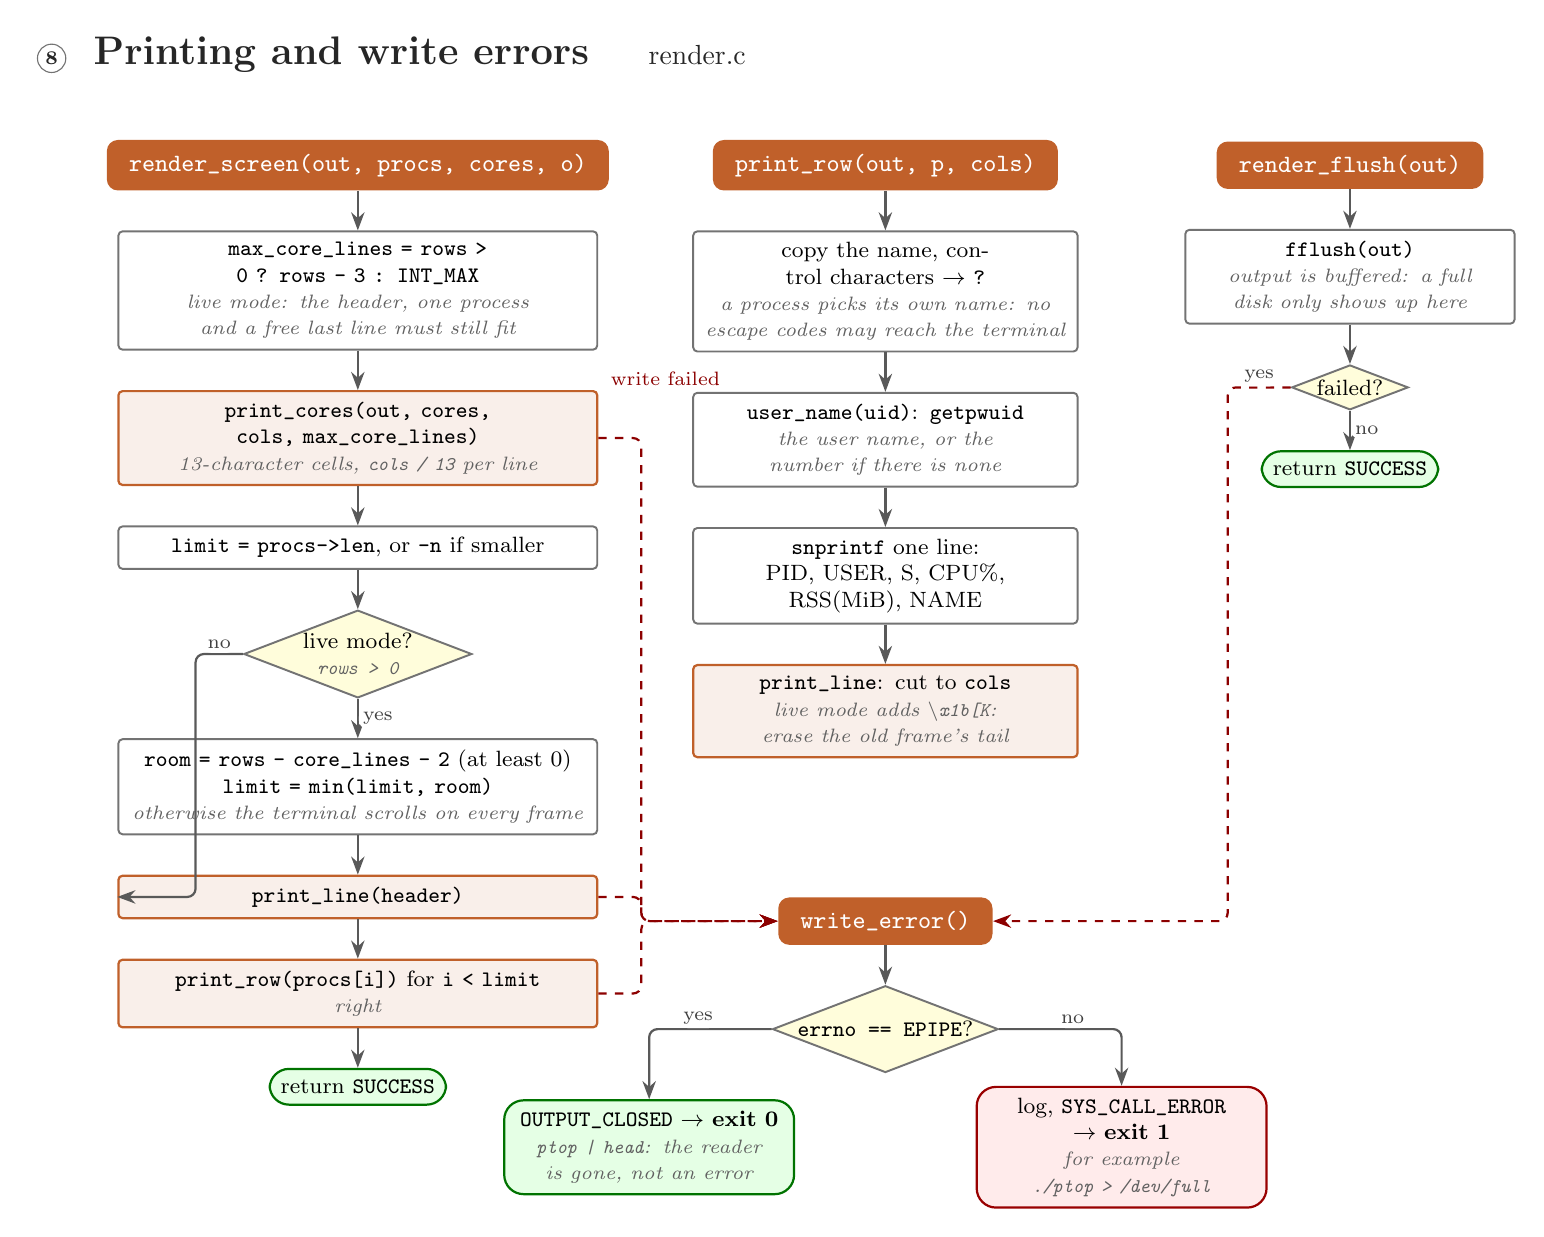
\begin{tikzpicture}[node distance=5mm and 8mm]
\node[pagehead] at (-4.2,1.4) {\st{8}\; Printing and write errors \quad{\normalsize\mdseries render.c}};

\node[ftitle=printc] (t) at (0,0) {\fn{render_screen(out, procs, cores, o)}};
\begin{scope}[act/.append style={text width=5.8cm}]
\node[act, below=of t] (a1) {\fn{max_core_lines = rows > 0 ? rows - 3 : INT_MAX}\\\nt{live mode: the header, one process and a free last line must still fit}};
\node[call=printc, below=of a1] (a2) {\fn{print_cores(out, cores, cols, max_core_lines)}\\\nt{13-character cells, \fn{cols / 13} per line}};
\node[act, below=of a2] (a3) {\fn{limit = procs->len}, or \fn{-n} if smaller};
\node[ask, below=of a3] (q1) {live mode?\\\nt{\fn{rows > 0}}};
\node[act, below=of q1] (a4) {\fn{room = rows - core_lines - 2} (at least 0)\\\fn{limit = min(limit, room)}\\\nt{otherwise the terminal scrolls on every frame}};
\node[call=printc, below=of a4] (a5) {\fn{print_line(header)}};
\node[call=printc, below=of a5] (a6) {\fn{print_row(procs[i])} for \fn{i < limit}\\\nt{right}};
\end{scope}
\node[good, below=of a6] (r) {return \fn{SUCCESS}};
\foreach \a/\b in {t/a1,a1/a2,a2/a3,a3/q1,a4/a5,a5/a6,a6/r} \draw[flow] (\a) -- (\b);
\draw[flow] (q1) -- node[lbl,right]{yes} (a4);
\draw[flow] (q1.west) -- node[lbl,above]{no} ++(-6mm,0) |- (a5.west);


%% print_row
\node[ftitle=printc] (u) at (6.7,0) {\fn{print_row(out, p, cols)}};
\begin{scope}[act/.append style={text width=4.6cm}]
\node[act, below=of u] (b1) {copy the name, control characters $\to$ \fn{?}\\\nt{a process picks its own name: no escape codes may reach the terminal}};
\node[act, below=of b1] (b2) {\fn{user_name(uid)}: \fn{getpwuid}\\\nt{the user name, or the number if there is none}};
\node[act, below=of b2] (b3) {\fn{snprintf} one line:\\PID, USER, S, CPU\%, RSS(MiB), NAME};
\node[call=printc, below=of b3] (b4) {\fn{print_line}: cut to \fn{cols}\\\nt{live mode adds \esc{[K}: erase the old frame's tail}};
\end{scope}
\foreach \a/\b in {u/b1,b1/b2,b2/b3,b3/b4} \draw[flow] (\a) -- (\b);

%% render_flush
\node[ftitle=printc] (v) at (12.6,0) {\fn{render_flush(out)}};
\node[act, below=of v, text width=3.9cm] (c1) {\fn{fflush(out)}\\\nt{output is buffered: a full disk only shows up here}};
\node[ask, below=of c1] (s1) {failed?};
\node[good, below=of s1] (ok) {return \fn{SUCCESS}};
\draw[flow] (v) -- (c1);
\draw[flow] (c1) -- (s1);
\draw[flow] (s1) -- node[lbl,right]{no} (ok);

%% write_error
\node[ftitle=printc] (w) at (6.7,-9.6) {\fn{write_error()}};
\node[ask, below=of w] (s2) {\fn{errno == EPIPE}?};
\node[good, text width=3.4cm] (g) at ([xshift=-30mm,yshift=-15mm]s2) {\fn{OUTPUT_CLOSED} $\to$ \textbf{exit 0}\\\nt{\fn{ptop | head}: the reader is gone, not an error}};
\node[bad, text width=3.4cm] (b) at ([xshift=30mm,yshift=-15mm]s2) {log, \fn{SYS_CALL_ERROR} $\to$ \textbf{exit 1}\\\nt{for example \fn{./ptop > /dev/full}}};
\draw[flow] (w) -- (s2);
\draw[flow] (s2.west) -| node[lbl,pos=0.3,above]{yes} (g.north);
\draw[flow] (s2.east) -| node[lbl,pos=0.3,above]{no} (b.north);

\foreach \n in {a2,a5,a6} \draw[flow, dashed, red!55!black] (\n.east) -- (\n.east -| 3.6,0) |- (w.west);
\node[lbl, text=red!55!black, anchor=south west] at ([xshift=1mm]a2.north east) {write failed};
\draw[flow, dashed, red!55!black] (s1.west) -- node[lbl,above]{yes} ++(-8mm,0) |- (w.east);
\end{tikzpicture}

%% ====================================================================
%% Page 9: terminal
%% ====================================================================
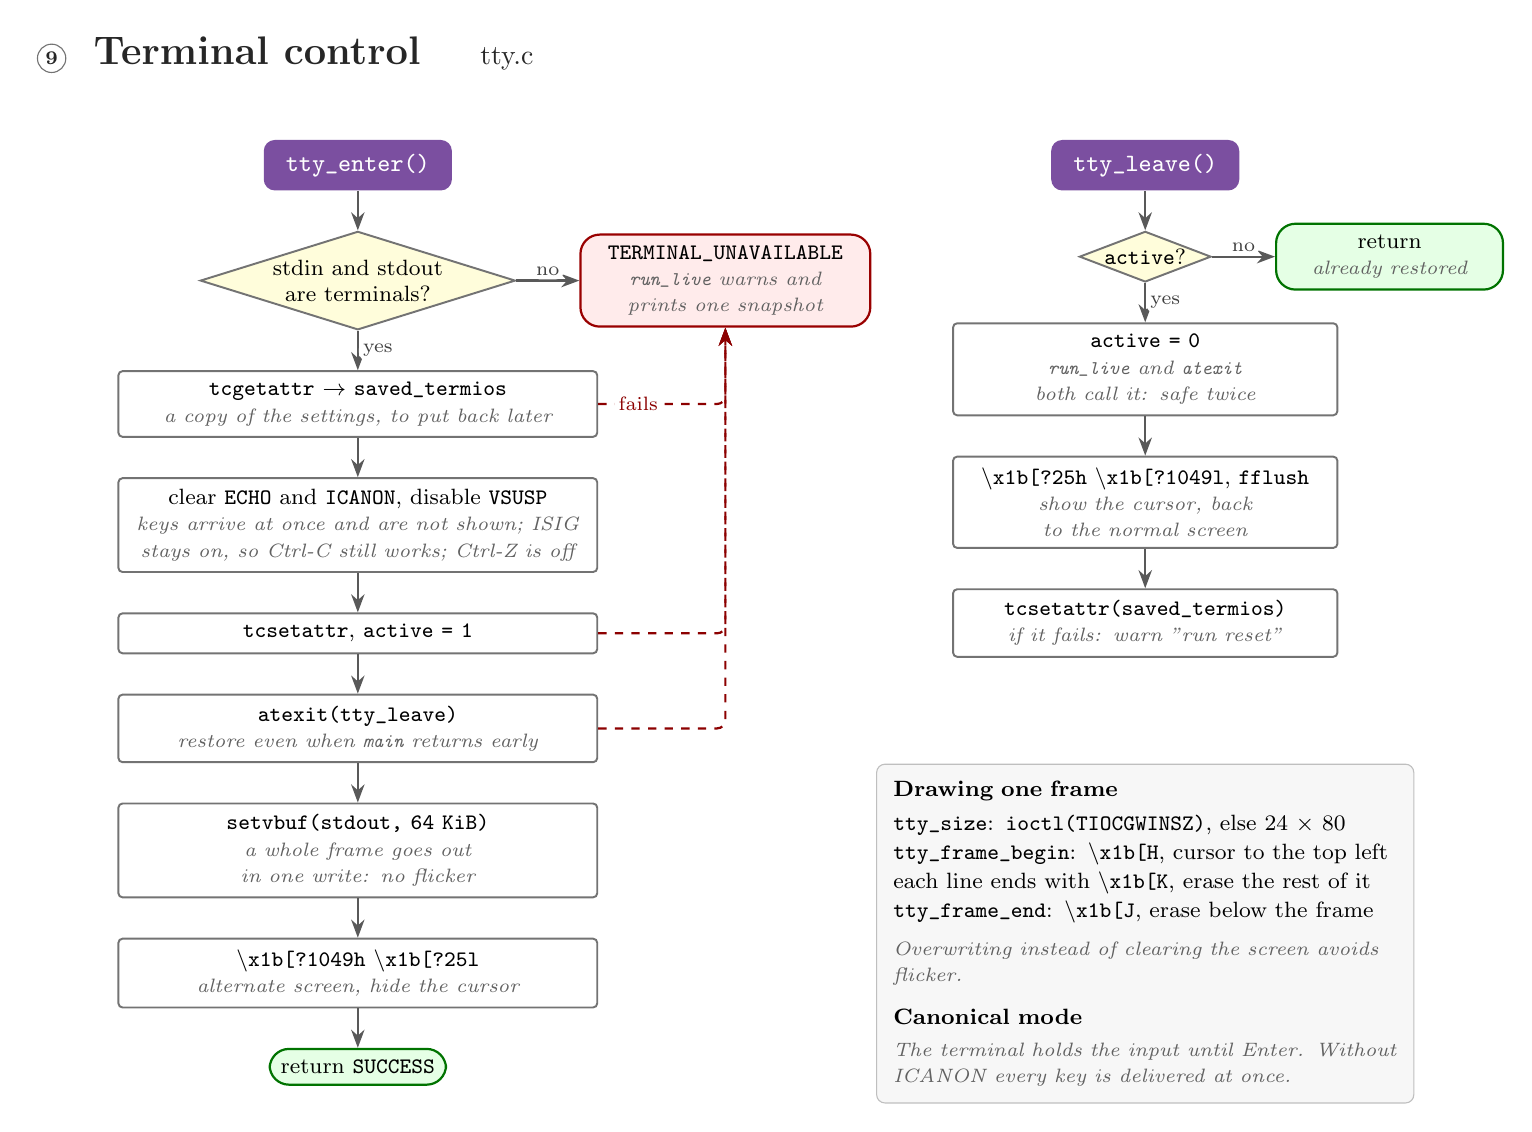
\begin{tikzpicture}[node distance=5mm and 8mm]
\node[pagehead] at (-4.2,1.4) {\st{9}\; Terminal control \quad{\normalsize\mdseries tty.c}};

\node[ftitle=ttyc] (t) at (0,0) {\fn{tty_enter()}};
\begin{scope}[act/.append style={text width=5.8cm}]
\node[ask, below=of t, aspect=3.2] (q1) {stdin and stdout\\are terminals?};
\node[act, below=of q1] (a1) {\fn{tcgetattr} $\to$ \fn{saved_termios}\\\nt{a copy of the settings, to put back later}};
\node[act, below=of a1] (a2) {clear \fn{ECHO} and \fn{ICANON}, disable \fn{VSUSP}\\\nt{keys arrive at once and are not shown; ISIG stays on, so Ctrl-C still works; Ctrl-Z is off}};
\node[act, below=of a2] (a3) {\fn{tcsetattr}, \fn{active = 1}};
\node[act, below=of a3] (a4) {\fn{atexit(tty_leave)}\\\nt{restore even when \fn{main} returns early}};
\node[act, below=of a4] (a5) {\fn{setvbuf(stdout, 64 KiB)}\\\nt{a whole frame goes out in one write: no flicker}};
\node[act, below=of a5] (a6) {\esc{[?1049h} \esc{[?25l}\\\nt{alternate screen, hide the cursor}};
\end{scope}
\node[good, below=of a6] (r) {return \fn{SUCCESS}};
\node[bad, right=of q1, text width=3.4cm] (x) {\fn{TERMINAL_UNAVAILABLE}\\\nt{\fn{run_live} warns and prints one snapshot}};
\foreach \a/\b in {t/q1,a1/a2,a2/a3,a3/a4,a4/a5,a5/a6,a6/r} \draw[flow] (\a) -- (\b);
\draw[flow] (q1) -- node[lbl,right]{yes} (a1);
\draw[flow] (q1) -- node[lbl,above]{no} (x);
\foreach \n in {a1,a3,a4} \draw[flow, dashed, red!55!black] (\n.east) -| (x.south);
\node[lbl, text=red!55!black, anchor=west] at ([xshift=2mm]a1.east) {fails};

%% tty_leave
\node[ftitle=ttyc] (u) at (10.0,0) {\fn{tty_leave()}};
\node[ask, below=of u] (p1) {\fn{active}?};
\node[good, right=of p1, text width=2.6cm] (y) {return\\\nt{already restored}};
\begin{scope}[act/.append style={text width=4.6cm}]
\node[act, below=of p1] (b1) {\fn{active = 0}\\\nt{\fn{run_live} and \fn{atexit} both call it: safe twice}};
\node[act, below=of b1] (b2) {\esc{[?25h} \esc{[?1049l}, \fn{fflush}\\\nt{show the cursor, back to the normal screen}};
\node[act, below=of b2] (b3) {\fn{tcsetattr(saved_termios)}\\\nt{if it fails: warn "run reset"}};
\end{scope}
\draw[flow] (u) -- (p1);
\draw[flow] (p1) -- node[lbl,above]{no} (y);
\draw[flow] (p1) -- node[lbl,right]{yes} (b1);
\draw[flow] (b1) -- (b2);
\draw[flow] (b2) -- (b3);

\node[side=6.4cm, anchor=north] at (10.0,-7.6) {%
  \textbf{Drawing one frame}\\[3pt]
  \fn{tty_size}: \fn{ioctl(TIOCGWINSZ)}, else 24 $\times$ 80\\[1pt]
  \fn{tty_frame_begin}: \esc{[H}, cursor to the top left\\[1pt]
  each line ends with \esc{[K}, erase the rest of it\\[1pt]
  \fn{tty_frame_end}: \esc{[J}, erase below the frame\\[4pt]
  \nt{Overwriting instead of clearing the screen avoids flicker.}\\[6pt]
  \textbf{Canonical mode}\\[2pt]
  \nt{The terminal holds the input until Enter. Without ICANON every key is delivered at once.}};
\end{tikzpicture}

%% ====================================================================
%% Page 10: live mode
%% ====================================================================
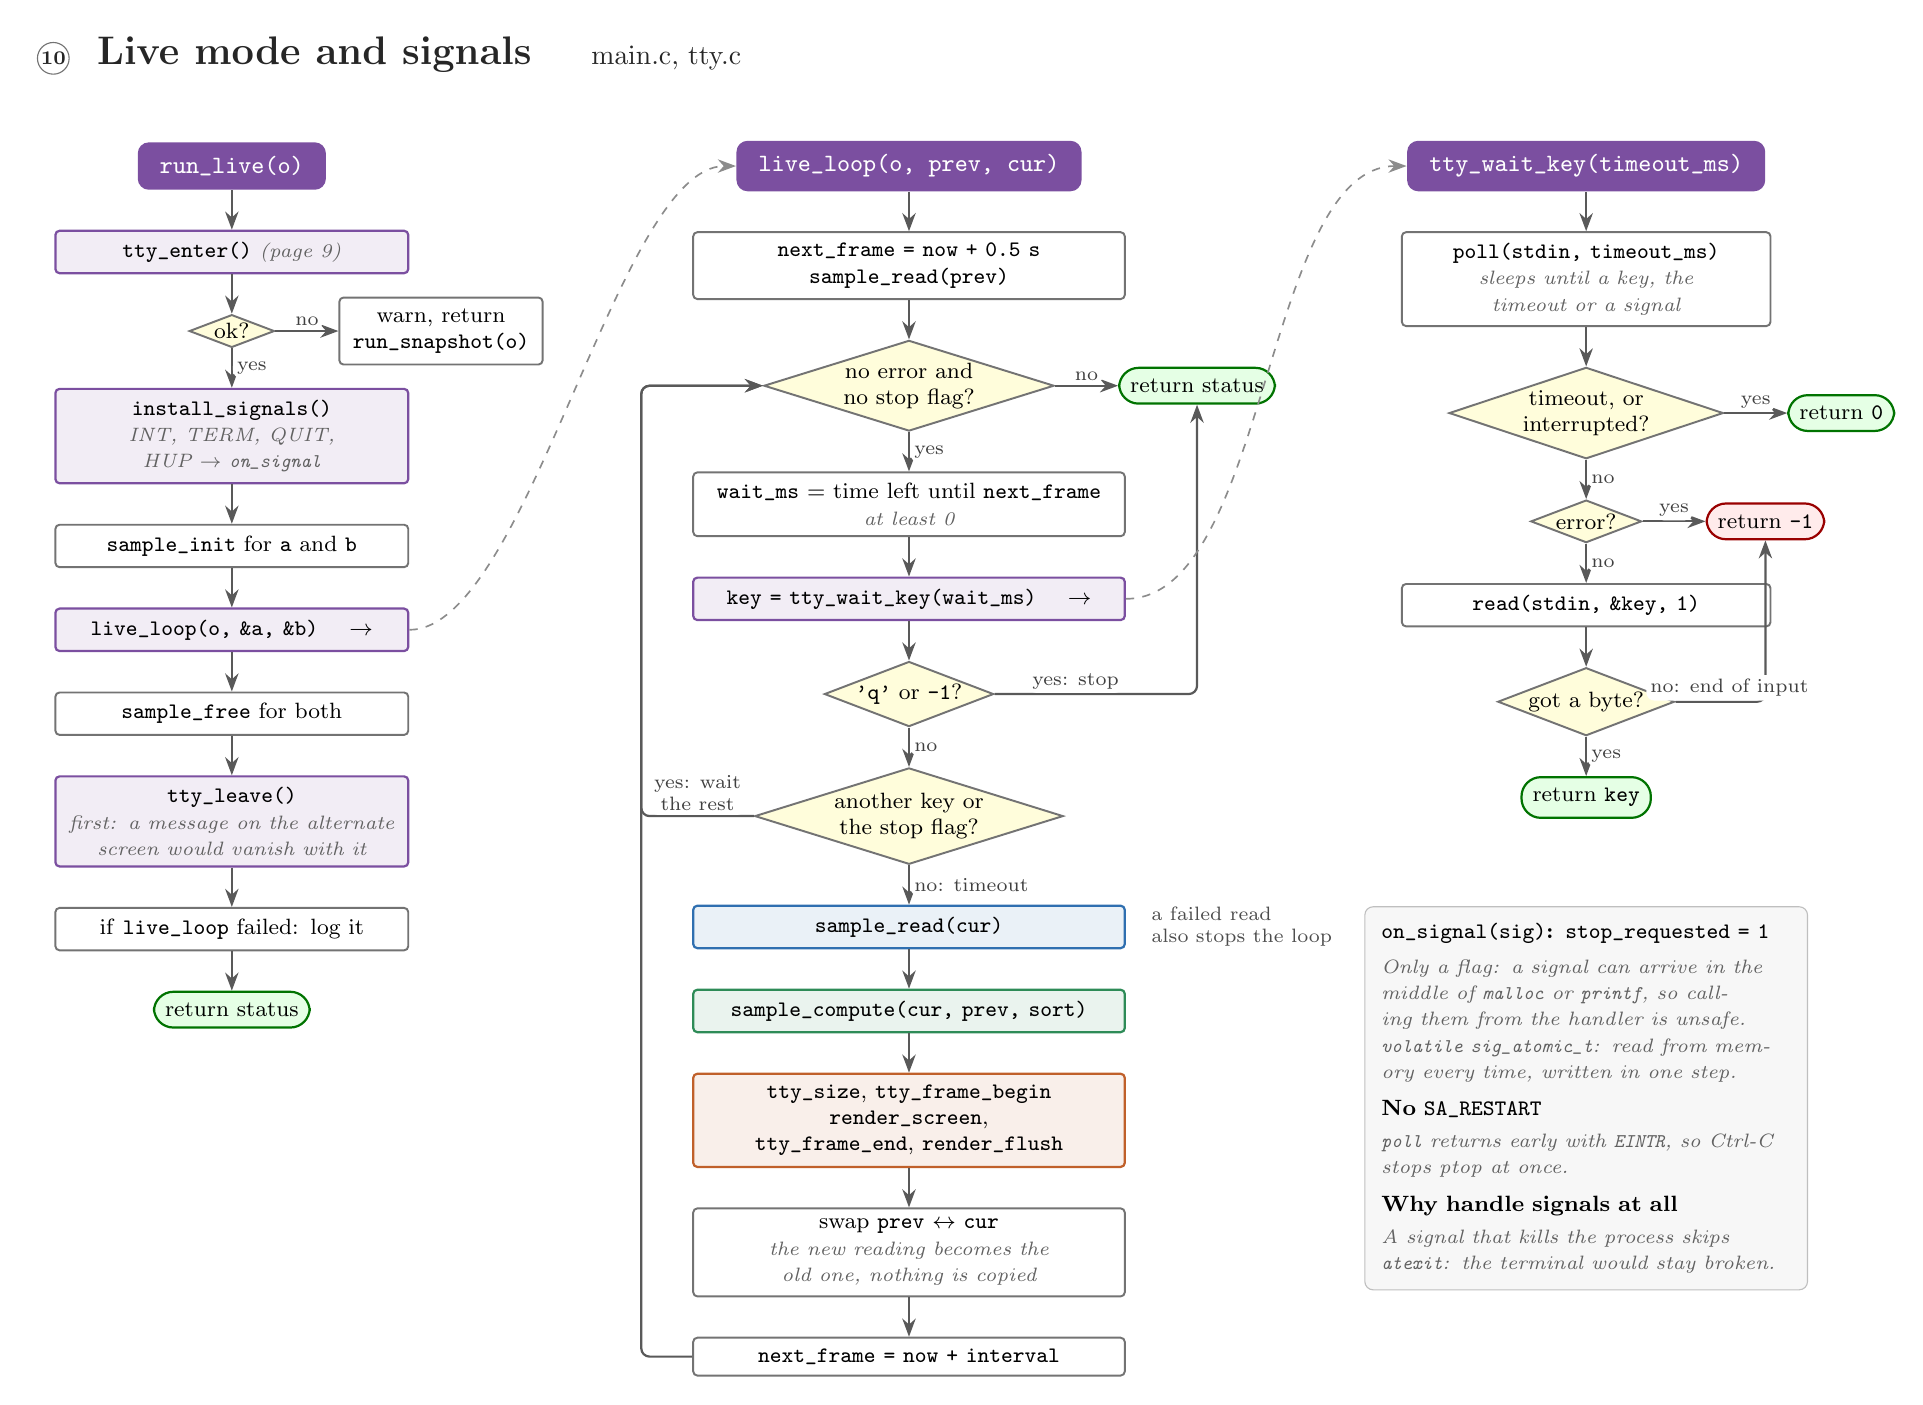
\begin{tikzpicture}[node distance=5mm and 8mm]
\node[pagehead] at (-11.2,1.4) {\st{10}\; Live mode and signals \quad{\normalsize\mdseries main.c, tty.c}};
\coordinate (L) at (-3.4,0);

%% run_live
\node[ftitle=ttyc] (s) at (-8.6,0) {\fn{run_live(o)}};
\begin{scope}[act/.append style={text width=4.2cm}]
\node[call=ttyc, below=of s] (c1) {\fn{tty_enter()} \nt{(page 9)}};
\node[ask, below=of c1] (k1) {ok?};
\node[call=ttyc, below=of k1] (c2) {\fn{install_signals()}\\\nt{INT, TERM, QUIT, HUP $\to$ \fn{on_signal}}};
\node[act, below=of c2] (c3) {\fn{sample_init} for \fn{a} and \fn{b}};
\node[call=ttyc, below=of c3] (c4) {\fn{live_loop(o, &a, &b)} \quad$\to$};
\node[act, below=of c4] (c5) {\fn{sample_free} for both};
\node[call=ttyc, below=of c5] (c6) {\fn{tty_leave()}\\\nt{first: a message on the alternate screen would vanish with it}};
\node[act, below=of c6] (c7) {if \fn{live_loop} failed: log it};
\end{scope}
\node[good, below=of c7] (c8) {return status};
\foreach \a/\b in {s/c1,c1/k1,c2/c3,c3/c4,c4/c5,c5/c6,c6/c7,c7/c8} \draw[flow] (\a) -- (\b);
\draw[flow] (k1) -- node[lbl,right]{yes} (c2);
\node[act, text width=2.3cm, right=of k1] (fb) {warn, return\\\fn{run_snapshot(o)}};
\draw[flow] (k1) -- node[lbl,above]{no} (fb);

%% live_loop
\node[ftitle=ttyc] (t) at (0,0) {\fn{live_loop(o, prev, cur)}};
\begin{scope}[act/.append style={text width=5.2cm}]
\node[act, below=of t] (a1) {\fn{next_frame = now + 0.5 s}\\\fn{sample_read(prev)}};
\node[ask, below=of a1, aspect=3.2] (q1) {no error and\\no stop flag?};
\node[act, below=of q1] (a2) {\fn{wait_ms} = time left until \fn{next_frame}\\\nt{at least 0}};
\node[call=ttyc, below=of a2] (a3) {\fn{key = tty_wait_key(wait_ms)} \quad$\to$};
\node[ask, below=of a3] (q2) {\fn{'q'} or \fn{-1}?};
\node[ask, below=of q2, aspect=3.2] (q3) {another key or\\the stop flag?};
\node[call=readc, below=of q3] (a4) {\fn{sample_read(cur)}};
\node[call=compc, below=of a4] (a5) {\fn{sample_compute(cur, prev, sort)}};
\node[call=printc, below=of a5] (a6) {\fn{tty_size}, \fn{tty_frame_begin}\\\fn{render_screen}, \fn{tty_frame_end}, \fn{render_flush}};
\node[act, below=of a6] (a7) {swap \fn{prev} $\leftrightarrow$ \fn{cur}\\\nt{the new reading becomes the old one, nothing is copied}};
\node[act, below=of a7] (a8) {\fn{next_frame = now + interval}};
\end{scope}
\node[good, right=of q1] (r) {return status};
\foreach \a/\b in {t/a1,a1/q1,a2/a3,a3/q2,a4/a5,a5/a6,a6/a7,a7/a8} \draw[flow] (\a) -- (\b);
\draw[flow] (q1) -- node[lbl,right]{yes} (a2);
\draw[flow] (q1) -- node[lbl,above]{no} (r);
\draw[flow] (q2) -- node[lbl,right]{no} (q3);
\draw[flow] (q3) -- node[lbl,right]{no: timeout} (a4);
\draw[flow] (q2.east) -| node[lbl,pos=0.2,above]{yes: stop} (r.south);
\draw[flow] (q3.west) -- node[lbl,above,pos=0.5,align=center]{yes: wait\\the rest} (q3.west -| L) |- (q1.west);
\draw[flow] (a8.west) -- (a8.west -| L) |- (q1.west);
\node[font=\scriptsize, text=black!70, anchor=west, align=left] at ([xshift=2mm]a4.east) {a failed read\\also stops the loop};

%% tty_wait_key
\node[ftitle=ttyc] (u) at (8.6,0) {\fn{tty_wait_key(timeout_ms)}};
\begin{scope}[act/.append style={text width=4.4cm}]
\node[act, below=of u] (b1) {\fn{poll(stdin, timeout_ms)}\\\nt{sleeps until a key, the timeout or a signal}};
\node[ask, below=of b1, aspect=3] (p1) {timeout, or\\interrupted?};
\node[ask, below=of p1] (p2) {error?};
\node[act, below=of p2] (b2) {\fn{read(stdin, &key, 1)}};
\node[ask, below=of b2] (p3) {got a byte?};
\end{scope}
\node[good, right=of p1] (g0) {return \fn{0}};
\node[bad, right=of p2] (g1) {return \fn{-1}};
\node[good, below=of p3] (g2) {return \fn{key}};
\draw[flow] (u) -- (b1);
\draw[flow] (b1) -- (p1);
\draw[flow] (p1) -- node[lbl,above]{yes} (g0);
\draw[flow] (p1) -- node[lbl,right]{no} (p2);
\draw[flow] (p2) -- node[lbl,above]{yes} (g1);
\draw[flow] (p2) -- node[lbl,right]{no} (b2);
\draw[flow] (b2) -- (p3);
\draw[flow] (p3) -- node[lbl,right]{yes} (g2);
\draw[flow] (p3.east) -| node[lbl,pos=0.3,above,align=center]{no: end of input} (g1.south);

\node[side=5.2cm, anchor=north] at (8.6,-9.4) {%
  \textbf{\fn{on_signal(sig)}: \fn{stop_requested = 1}}\\[3pt]
  \nt{Only a flag: a signal can arrive in the middle of \fn{malloc} or \fn{printf}, so calling them from the handler is unsafe.
  \fn{volatile sig_atomic_t}: read from memory every time, written in one step.}\\[4pt]
  \textbf{No \fn{SA_RESTART}}\\[2pt]
  \nt{\fn{poll} returns early with \fn{EINTR}, so Ctrl-C stops ptop at once.}\\[4pt]
  \textbf{Why handle signals at all}\\[2pt]
  \nt{A signal that kills the process skips \fn{atexit}: the terminal would stay broken.}};
\draw[black!45, dashed, ->, line width=0.6pt] (c4.east) .. controls +(1.5,0) and +(-1.5,0) .. (t.west);
\draw[black!45, dashed, ->, line width=0.6pt] (a3.east) .. controls +(1.8,0) and +(-1.8,0) .. (u.west);
\end{tikzpicture}

\end{document}
